% edbktmpl.tex. Current Version: June 5, 1999
%%%%%%%%%%%%%%%%%%%%%%%%%%%%%%%%%%%%%%%%%%%%%%%%%%%%%%%%%%%%%%%%
%
%  Template file for
%  Wiley edited book
%  Wiley Book Style, Design No.: SD 001E
%
%  Prepared by Amy Hendrickson, TeXnology Inc., March 1996.
%%%%%%%%%%%%%%%%%%%%%%%%%%%%%%%%%%%%%%%%%%%%%%%%%%%%%%%%%%%%%%%%

%%%%%%%%%%%%%%%%
% LaTeX2e:
 \documentclass{w-edbk}

    % For TimesRoman Math (You must have MathTimes and MathTimes Plus 
    %                        font sets, order fonts from  www.yandy.com)
%\usepackage[mtbold,noTS1]{m-times}

    % For PostScript text, Computer Modern Math 
    
\usepackage{w-edbkps}

%%%%%%%%%%%%%%%%
% LaTeX2.09:
% \documentstyle{w-edbk}
    % For PostScript text, Computer Modern Math
% \documentstyle[w-edbkps]{w-edbk} 
    % For MathTimes and PostScript:
    %(m-times only works with LaTeX2e)

%%%%%%%%%%%%%%%%%%%%%%%%%%%%%%
%% Change options here if you want:
%%
%% How many levels of section head would you like numbered?
%% 0= no section numbers, 1= section, 2= subsection, 3= subsubsection
%%==>>
\setcounter{secnumdepth}{1}

%% How many levels of section head would you like to appear in the
%% Table of Contents?
%% 0= chapter titles, 1= section titles, 2= subsection titles, 
%% 3= subsubsection titles.
%%==>>
\setcounter{tocdepth}{1}
%%%%%%%%%%%%%%%%%%%%%%%%%%%%%%
%
% DRAFT
%
% Uncomment to get double spacing between lines, current date and time
% printed at bottom of page.
% \draft
% (If you want to keep tables from becoming double spaced also uncomment
% this):
% \renewcommand{\arraystretch}{0.6}
%%%%%%%%%%%%%%%%%%%%%%%%%%%%%%

\usepackage{url}
\usepackage[round]{natbib}
\usepackage{graphicx}
\usepackage{amsmath}
\usepackage{amssymb}
\usepackage{bbm}

%% Our own commands
\newcommand{\ignore}[1]{}
\newcommand{\textR}{\raisebox{.6ex}{\scriptsize \textregistered}}
\newcommand{\eps}{\varepsilon}
\newcommand{\Ind}[1]{\mathbbm{1}_{\{{#1}\}}}
\newcommand{\optional}[1]{}
\newcommand{\Greedyplus}{Greedy+}

%% %%%%%%%%%%%%%%%%%%%%%%%%%%%%%%%%%%%%%%%%%%%%%%%%%%%%%%%%%%%%%%%%%%%%%%%%%%%%%
%% Notation
%% --------
%%
%% n: number of probes
%% m: number of spots
%% t: step index
%% N: deposition sequence
%% N_t: nucleotide added at step t
%% M_t: mask of step t
%% T: total number of synthesis steps
%%
%% s,s': spot indices
%% p_k: probe sequence of probe with index k
%% k(s): probe index for spot s
%% \eps_k: embedding vector for probe with index k
%% \eps_{k(s)}: embedding vector at spot s
%%
%% \mathcal{B}_t: border length of mask M_t
%%
%% For the QAP formulation (not here!)
%% k,l: indices for probes
%% i,j: indices for spots
%%
%% %%%%%%%%%%%%%%%%%%%%%%%%%%%%%%%%%%%%%%%%%%%%%%%%%%%%%%%%%%%%%%%%%%%%%%%%%%%%%


\begin{document}

%% To be entered at Wiley, for final production: title page information,
%% table of contents, preface and introduction, and Part titles, and index. 
%% See edbksamp.tex for examples of how to enter the commands.

% \footnote{text} will cause a footnote to appear at the bottom of the page.

%% 
\title[Algorithms for Microarray Layout]{Algorithms for Oligonucleotide Microarray Layout}

%% Please supply author names in upper and lower case within square
%% brackets and in uppercase in curly brackets, i.e.,
%% \author[The Author]{THE AUTHOR\footnote{Presently on leave at
%% NASA, Houston, Texas, USA.}}
%% You may use a footnote for additional information.

\author[S\'ergio A.~de~Carvalho~Jr. and Sven Rahmann]{S\'ERGIO A.~DE~CARVALHO~JR. and SVEN RAHMANN}

%\affil{AT\& T Bell Laboratories\\
%Murray Hill, New Jersey}

\affil{%%
Algorithms and Statistics for Systems Biology, Genome Informatics, \\
Technische Fakult\"at, Bielefeld University, D-33594 Bielefeld, Germany\\
\url{Sergio.Carvalho@cebitec.uni-bielefeld.de}\\
\url{Sven.Rahmann@cebitec.uni-bielefeld.de}\\
}

% prologue is optional. First arg is for text, second for author attribution.
% May be indexed and/or referenced. i.e.,

%\prologue{The sheer volume of answers can often stifle insight...The purpose
%of computing\inxx{computing,the purpose} is insight, not numbers.}
%{Hamming}

%\prologue{}{}

%% Article text:

Microarrays are a ubiquitous tool in molecular biology with a
wide range of applications on a whole-genome scale including
high-throughput gene expression analysis, genotyping, and resequencing.
The advantage of oligonucleotide arrays is that their higher densities
allow, for instance, the simultaneous measurement of the expression of
several thousand genes at once. High-density microarrays are usually
produced by light-directed combinatorial chemistry that builds the
probe sequences base-by-base. Because of the natural properties of
light, the quality of a microarray can be improved by carefully
designing the physical arrangement, or \emph{layout}, of its probes.
In this chapter, we review models for evaluating the layout of
oligonucleotide microarrays and survey algorithmic approaches
that can be used in their design.

%%%%%%%%%%%%%%%%%%%%%%%%%%%%%%%%%%%%%%%%%%%%%%%%%%%%%%%%%%%%%%%%%%%%%%%%%%%%%%%%
\section{Introduction}
\label{sec:intro}

Oligonucleotide microarrays consist of short DNA fragments, called
\emph{probes}, affixed or synthesized at specific locations, called
\emph{features} or \emph{spots}, of a solid surface. Microarrays are
based on the principle of Watson-Crick base pairing. Each probe is a
single-stranded DNA molecule of 10 to 70 nucleotides that perfectly matches
with a specific part of a \emph{target} molecule. The probes are used to
verify whether (or in which quantity) the targets are present in a
given biological sample.

\ignore{
This type of microarray was originally designed in the late 1980s as a tool for
DNA sequencing, a technology that is known as DNA Sequencing by Hybridization.
}

The first step of a microarray experiment consists of collecting mRNAs
or genomic DNA from the cells or tissue under investigation. The mixture
to be analyzed is prepared with fluorescent tags and loaded on the array,
allowing
the targets to hybridize with the probes. Any unbound molecule is
washed away, leaving on the array only those molecules that have found
a complementary probe. Finally, the array is exposed to a light source
that induces fluorescence, and an optical scanner reads the intensity
of light emitted at each spot.

Under ideal conditions, each probe will hybridize only to its target.  Thus,
it is possible to infer whether a given molecule is present in the sample by
checking whether there is light coming from the corresponding spot of the
array.  The expression level of a gene in a cell can also be inferred because
each spot contains several million identical probes, and the strength of the
fluorescent signal on a spot is expected to be proportional to the
concentration of the target in the sample. In practice, each target is queried
by several probes (its \emph{probe set}), and complex statistical calculations
are performed to infer the concentration from the observed signals.

High-density microarrays, also called microarray chips, can have more than a
million spots, and are thus able to query tens of thousands of genes, covering
the entire genome of an organism.  The pioneering Affymetrix GeneChip\textR\ 
arrays, for instance, have up to 1.3~million spots on a coated quartz
substrate measuring a little over 1~cm$^2$.  The spots are as narrow as
5~$\mu$m (5~microns, or 0.005 mm), and are arranged in a regularly-spaced
rectangular grid.

\subsection{Microarray production}

GeneChip arrays are produced by combinatorial chemistry and techniques derived
from micro-electronics and integrated circuits fabrication. Probes are typically
25 bases long and are synthesized on the chip, in parallel, in a series of
repetitive steps. Each step appends the same kind of nucleotide to probes of
selected
regions of the chip. The selection of which probes receive the nucleotide is
achieved by a process called \emph{photolithography} \citep{Fodor1991}.

\begin{figure}\centering
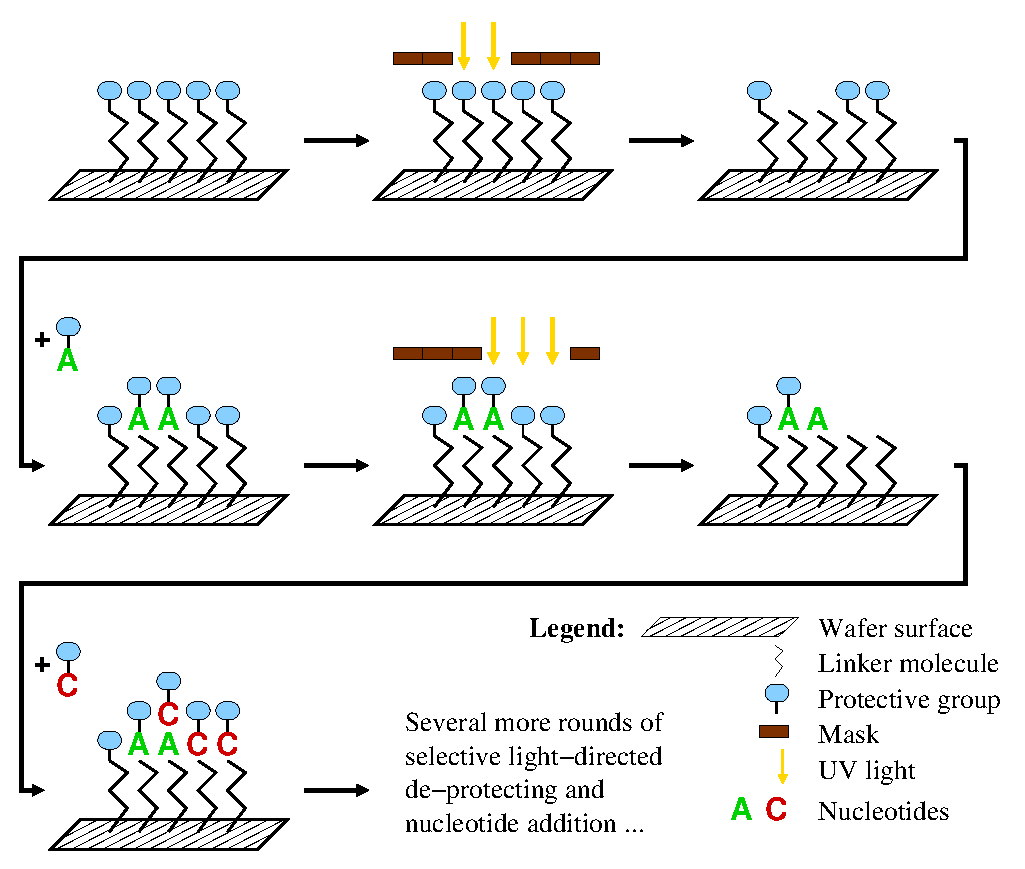
\includegraphics[width=.7\textwidth]{figures/production.eps}
\caption{Affymetrix's probe synthesis via photolithographic masks. The chip is
  coated with a chemical compound and a light-sensitive protecting group;
  masks are used to direct light and activate selected probes for chemical
  coupling; nucleotides are appended to deprotected probes; the process is
  repeated until all probes have been fully synthesized.}
\label{fig:photolithography}
\end{figure}

Figure~\ref{fig:photolithography} illustrates this process: The quartz
wafer of a GeneChip array is initially coated with a chemical compound
topped with a light-sensitive protecting group that is removed when
exposed to ultraviolet light, activating the compound for chemical
coupling. A lithographic mask is used to direct light and remove the
protecting groups of only those positions that should receive the
nucleotide of a particular synthesis step.  A solution containing
adenine (A), thymine (T), cytosine (C) or guanine (G) is then flushed
over the chip surface, but the chemical coupling occurs only in those
positions that have been previously deprotected. Each coupled
nucleotide also bears another protecting group so that the process can
be repeated until all probes have been fully synthesized.



Photolithographic masks are notoriously expensive and cannot be changed once
they have been manufactured. Thus, any change in the chip layout requires the
production of a new set of masks. A similar method of \emph{in situ} synthesis
known as Maskless Array Synthesizer (MAS) was later developed to eliminate the
need of such masks \citep{Singh-Gasson1999}. Probes are still built by
repeating cycles of deprotection and chemical coupling of nucleotides. The
illumination, however, relies on an array of miniature mirrors that can be
independently controlled to direct or deflect the incidence of light on the
chip.

NimbleGen Systems, Inc.\ uses its own Digital Micromirror Device (DMD) that
can control up to 786\,000 individual mirrors to produce microarrays with
spots as small as 16 $\mu$m $\times$ 16 $\mu$m. The Geniom\textR\ system of
febit biotech GmbH, a platform for customized microarray production, also uses
a micromirror array to direct the synthesis process.


\subsection{The problem of unintended illumination}

Regardless of which method is used to direct light (masks or micromirror
arrays), it is possible that some probes are accidentally activated for
chemical coupling because of light diffraction, scattering or internal
reflection on the chip surface. This unwanted illumination of regions
introduces unexpected nucleotides that change probe sequences,
significantly reducing their chances of successful hybridization with their
targets. Moreover, these faulty probes may also introduce
cross-hybridizations, which can interfere in the experiments performed with
the chip.

This problem is more likely to occur near the borders between a masked and
an unmasked spot (in the case of maskless synthesis, between a spot that
is receiving light and a spot that is not). This observation has given rise to
the term \emph{border conflict}.

It turns out that by carefully designing the \emph{arrangement} of the probes
on the chip and their \emph{embeddings} (the sequences of masked and unmasked
steps used to synthesize each probe), it is possible to reduce the risk of
unintended illumination. This issue becomes even more important as there is a
need to accommodate more probes on a single chip, which requires the
production of spots at higher densities and, consequently, with reduced
distances between probes.

In this chapter, we address the problem of designing the layout of a
microarray with the goal of reducing the chances of unintended illumination,
which we call Microarray Layout Problem (MLP). We use the term \emph{layout}
to refer to where and how the probes are synthesized on the chip (their
arrangement and their embeddings).


%%%%%%%%%%%%%%%%%%%%%%%%%%%%%%%%%%%%%%%%%%%%%%%%%%%%%%%%%%%%%%%%%%%%%%%%%%%%%%%%
\section{The Microarray Layout Problem}
\label{sec:eval}

In this section we give a more precise definition of the Microarray Layout
Problem (MLP) and define criteria for evaluating a given layout. The description
that follows assumes that synthesis is done by photolithographic masks, but the
concepts apply to the maskless production as well. Two evaluation criteria are
presented: \emph{border length} and \emph{conflict index}. As shown
later, the conflict index model can be seen as a generalization of the border
length model.

Formally, we have a set of probes $\mathcal{P} = \{p_{1}, p_{2},
\dots, p_{n}\}$ (frequently, but not necessarily, all probes have the
same length), where each $p_k \in \{\text{A,C,G,T}\}^\ast$ is
produced by a series of $T$ synthesis steps. Each step $t$ uses a mask
$M_t$ to induce the addition of a particular nucleotide $N_t \in
\{\text{A,C,G,T}\}$ to a subset of~$\mathcal{P}$
(Fig.~\ref{fig:masking_process}).  The \emph{nucleotide deposition
  sequence} $N = N_{1} N_{2} \ldots N_{T}$ corresponding to the
sequence of nucleotides added at each synthesis step is therefore a
supersequence of all $p \in \mathcal{P}$.

A microarray chip consists of a set of spots, or sites, $\mathcal{S} =
\{s_{1}, s_{2}, \dots, s_{m}\}$, where each spot $s$ is specified by its
coordinates on the chip surface and accommodates a unique probe
$p_k \in \mathcal{P}$. Note that we usually refer to $s$ as
containing a single probe $p_k$ although, in practice, it
contains several million copies of it. Each probe is synthesized at a
unique spot, hence there is a one-to-one assignment between probes and
spots (if we assume that there are as many spots as probes, i.e.,
$m=n$).

In general, a probe can be \emph{embedded} within $N$ in several ways.
An embedding of $p_{k}$ is a $T$-tuple $\eps_{k} = (\eps_{k,1},
\eps_{k,2}, \dots, \eps_{k,T})$ in which $\eps_{k,t} = 1$ if probe
$p_{k}$ receives nucleotide $N_{t}$ (at step~$t$), and 0 otherwise.  In
particular, a \emph{left-most embedding} is an embedding in which the
bases are added as early as possible (as in $\eps_1$ in
Fig.~\ref{fig:masking_process}).  We say that a spot or an embedding
$\eps_k$ is \emph{productive} (unmasked) at step $t$ if $\eps_{k,t} =
1$, or \emph{unproductive} (masked) otherwise.


\begin{figure}
\centerline{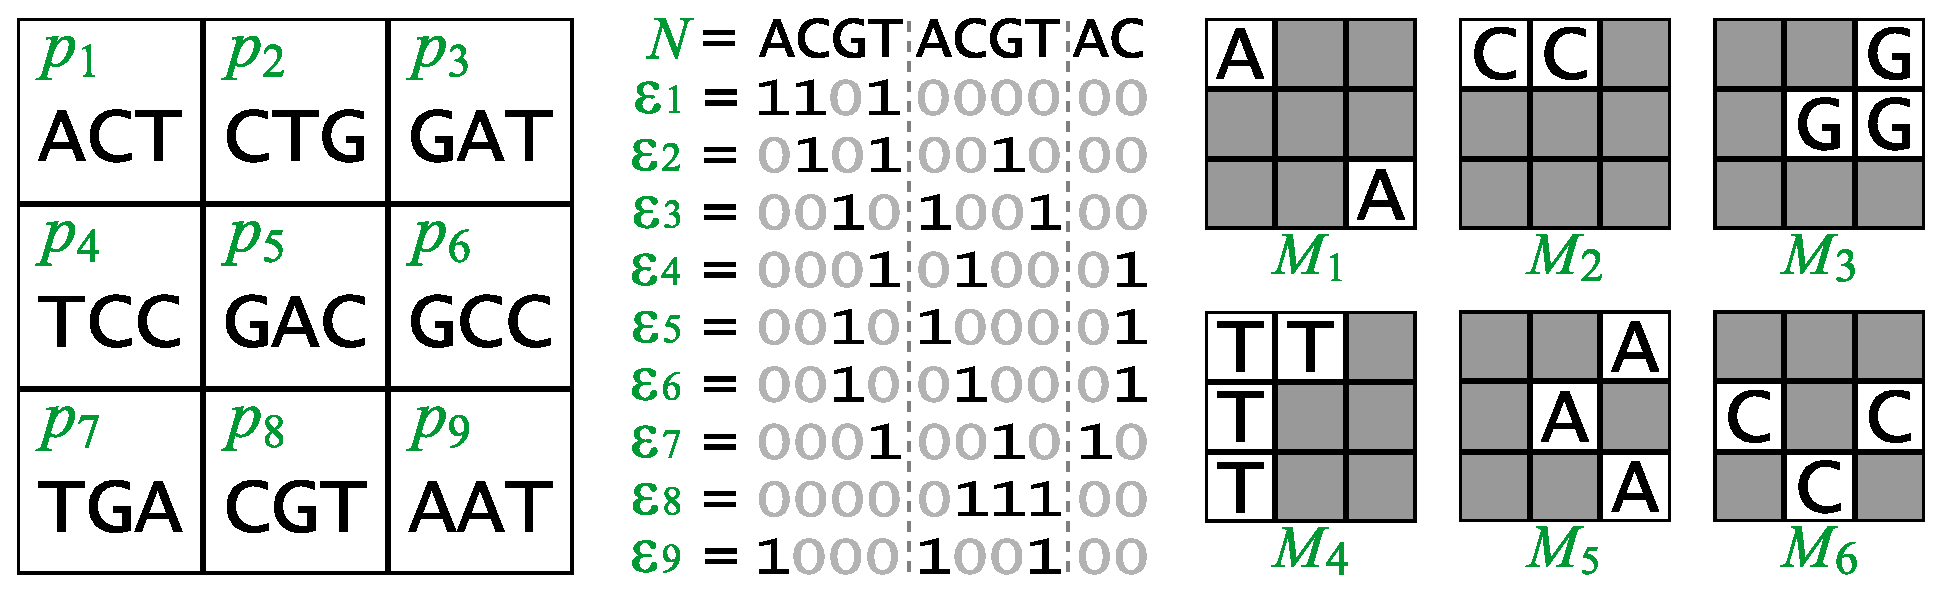
\includegraphics[width=\textwidth]{figures/chip.eps}}
\caption{Synthesis of a hypothetical 3$\times$3 chip with photolithographic
masks. Left: chip layout and the 3-mer probe sequences. Center: deposition
sequence and probe embeddings. Right: first four masks.}
\label{fig:masking_process}
\end{figure}

The deposition sequence is often a repeated permutation of the alphabet, mainly
because of its regular structure and because such sequences maximize the number
of distinct subsequences \citep{Chase1976}. The deposition sequence shown in
Fig.~\ref{fig:masking_process} is a 2.5-time repetition of ACGT, and we thus
say that it has two and a half \emph{cycles}.

For cyclic deposition sequences, it is possible to distinguish between two
types of embeddings: \emph{synchronous} and \emph{asynchronous}. In the first
case, each probe has exactly one nucleotide synthesized in every cycle of the
deposition sequence; hence, 25 cycles or 100 steps are needed to synthesize
probes of length 25. In the case of asynchronous embeddings, probes can have
any number of nucleotides synthesized in any given cycle, allowing shorter
deposition sequences. For this reason, asynchronous embeddings are usually the
choice for commercial microarrays.  For instance, all GeneChip arrays are
asynchronously synthesized in 74~steps (18.5 cycles of TGCA), so only
sub-sequences of this particular deposition sequence can be selected as probes
on Affymetrix chips.  \citet{Rahmann2006SubsequenceCombinatorics} shows that
this covers about 98.45\% of all 25-mers.

Ideally, the deposition sequence should be as short as possible in order to
reduce manufacturing time, cost and probability of errors \citep{Rahmann2003}.
Finding the shortest deposition sequence to synthesize a set of probes is an
instance of a classical computer science problem known as the Shortest Common
Supersequence problem. Here, however, we assume that $N$ is a fixed sequence
given as input.


\subsection{Problem statement}

Given a set of probes $\mathcal{P}$, a geometry of spots $\mathcal{S}$,
and a deposition sequence $N$ as specified above, the MLP asks to
specify a chip layout $(k,\eps)$ that consists of
\begin{enumerate}
\item a bijective assignment $k: \mathcal{S}\to \{1,\dots,n\}$ that
  specifies a probe index $k(s)$ for each spot $s$ (meaning that
  $p_{k(s)}$ will be synthesized at $s$),
\item an assignment $\eps: \{1,\dots,n\}\to \{0,1\}^T$ specifying an
  embedding $\eps_k = (\eps_{k,1},\dots,\eps_{k,T})$ for each
  probe index $k$, such that $N[\eps_k] :\equiv (N_t)_{t:
    \eps_{k,t}=1} = p_k$,
\end{enumerate}
such that a given penalty function is minimized.  We introduce two
such penalty functions: total border length and total conflict index.

%We may thus speak of $\eps_{k(s)}$ as the embedding at spot $s$.


\subsection{Border length}

A precursor of the MLP (that did not consider different embeddings)
was formally stated by Hannenhalli and co-workers \citep{Hannenhalli2002},
who defined
the \emph{border length}~$\mathcal{B}_t$ of a mask~$M_{t}$ as the
number of borders separating masked and unmasked spots at synthesis
step~$t$, that is, the number of border
conflicts in $M_{t}$. The total border length of a given layout is the
sum of border lengths over all masks. For example, the four masks
shown in Fig.~\ref{fig:masking_process} have $\mathcal{B}_1 = 4$,
$\mathcal{B}_2 = 3$, $\mathcal{B}_3 = 5$ and $\mathcal{B}_4 = 4$. The
total border length of that layout is 52 (masks 5 to 10 not shown).

The total border length is a possible penalty function to evaluate a
proposed layout, and the \emph{Border Length Minimization Problem}
(BLP) is then defined as the problem of finding a layout minimizing
total border length.


\subsection{Conflict index}

The border length measures the quality of an individual mask or set of masks.
With this model, however, it is not possible to know how the border conflicts
are distributed among the probes. Ideally, all probes should have roughly the
same risk of being damaged by unintended illumination, so that all signals are
affected by the resulting imperfections in approximately the same way.

The \emph{conflict index} is a quality measure defined with the aim of
estimating the risk of damaging probes at a particular spot
\citep{Carvalho2006a} -- it is a per-spot or per-probe measure instead
of a per-mask measure.  Additionally, it takes into account two
practical considerations observed by \citet{Kahng2003}:
%%
\begin{itemize}
\item[a)] stray light might activate not only adjacent neighbors but
  also spots that lie as far as three cells away from the targeted
  spot;
\item[b)] imperfections produced in the middle of a probe are more
  harmful than in its extremities.
\end{itemize}

For a proposed layout $(k,\eps)$, the conflict index~$\mathcal{C}(s)$
of a spot $s$ whose probe $p_{k(s)}$ is synthesized in $T$~masking
steps according to its embedding vector $\eps_{k(s)}$ is
%%
\begin{equation}
\label{eq:conf_idx}
\mathcal{C}(s) := \sum_{t=1}^{T} \Bigl(
  \Ind{\eps_{k(s),t}=0}
  \cdot \omega(\eps_{k(s)},t)
  \cdot \sum_{\substack{s'\text{: neighbor}\\\text{of } s}}
  \Ind{\eps_{k(s'),t}=1}
  \cdot \gamma(s,s') \Bigr),
\end{equation}
%%
where $\Ind{cond}$ is the indicator function that equals 1 if condition
$cond$ is true, and 0 otherwise. The indicator functions ensure the following
conflict condition: During step~$t$, there is a conflict at spot~$s$ if and
only if $s$ is masked ($\eps_{k(s),t}=0$) and a close neighbor
$s'$ is unmasked ($\eps_{k(s'),t}=1$), since light directed at
$s'$ may somehow reach $s$.  When $s$ is productive, it does not matter
if it accidentally receives light targeted at a neighbor, and when $s'$ is
unproductive, there is no risk that it damages probes of $s$.

Function $\gamma(s,s')$ is a ``closeness'' measure between $s$ and $s'$ (to
account for observation a). It is defined as
%%
\begin{equation}\label{eq:dist_weight}
\gamma(s,s') := (d(s,s'))^{-2},\nopagebreak
\end{equation}\nopagebreak
%%
where $d(s,s')$ is the Euclidean distance between the spots $s$ and $s'$. Note
that in (\ref{eq:conf_idx}), $s'$ ranges over all neighboring spots that are at
most three cells away (horizontally and vertically) from $s$ (see
Fig.~\ref{fig:conflictindex}~left), which is in accordance with observation a.

The position-dependent weighting function $\omega(\eps,t)$ accounts for
the significance of the location inside the probe where the undesired nucleotide
is introduced in case of accidental illumination (observation b). It is defined
as:
%%
\begin{equation}\label{eq:pos_mult}
\omega(\eps,t) := c \cdot \exp{\left(\theta \cdot \lambda(\eps,t)\right)}
\end{equation}
%%
where $c>0$ and $\theta>0$ are constants, and for $1\leq t\leq T$,
%%
\begin{equation}\label{eq:base_pos}
  \lambda(\eps,t) := 1 + \min(b_{\eps,t},\ell_{\eps} - b_{\eps,t}),
\end{equation}
%%
\begin{equation}\label{eq:b_ell}
  b_{\eps,t} := \sum_{t'=1}^{t} \eps_{t'},
  \qquad
  \ell_{\eps} := \sum_{t=1}^{T} \eps_t = b_{\eps,T}.
\end{equation}

In other words, $\ell_\eps$ is the length of the final probe specified
by $\eps$ (equal to the number of ones in the embedding), and
$b_{\eps,t}$ denotes the number of nucleotides synthesized up to and
including step~$t$.

Note that $\omega(\eps,t)$ grows exponentially from the extremities of the
probe to its center (see Fig.~\ref{fig:conflictindex} right). The motivation
behind this definition is that the probability of a successful stable
hybridization of a probe with its target should increase exponentially with
the absolute value of its Gibbs free energy, which increases linearly with the
length of the longest perfect match between probe and target. The parameter
$\theta$ controls how steeply the exponential weighting function rises towards
the middle of the probe. In Fig.~\ref{fig:conflictindex} and our experiments,
we use probes of length $\ell=25$, and parameters $\theta = 5/\ell$ and $c =
1/\exp{(\theta)}$.

%%
\ignore{It is generally agreed that the chances of a successful hybridization
  between probe and target are higher if a mismatched base occurs at the
  extremities of the formed duplex instead of at its center. The precise
  effects of this position, however, is not yet fully understood and has been
  an active topic of research \citep{BINDER05}.}
%%

\begin{figure}
%%
\begin{picture}(145,105)
  \put(0,0){\makebox(145,105){
    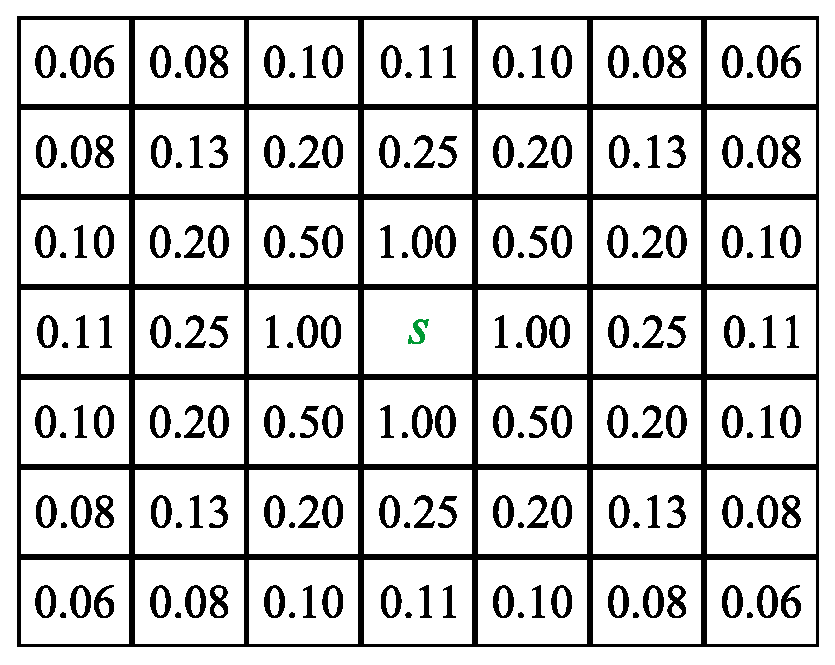
\includegraphics[width=0.4\textwidth]{figures/distweights}
  }}
\end{picture}
%%
\begin{picture}(190,105)
  \footnotesize{
    \put(0,0){\makebox(190,105){
      %GNUPLOT: LaTeX picture with Postscript
      \begin{picture}(0,0)%
      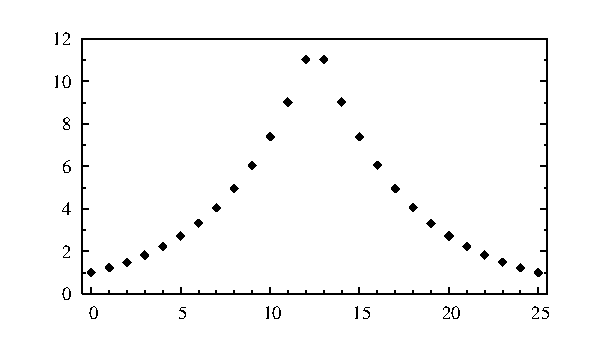
\includegraphics{figures/posweights}%
      \end{picture}%
      \begingroup
      \setlength{\unitlength}{0.0200bp}%
      \begin{picture}(9900,5940)(0,0)%
      \put(1250,1000){\makebox(0,0)[r]{\strut{} 0}}%
      \put(1250,1740){\makebox(0,0)[r]{\strut{} 2}}%
      \put(1250,2480){\makebox(0,0)[r]{\strut{} 4}}%
      \put(1250,3220){\makebox(0,0)[r]{\strut{} 6}}%
      \put(1250,3960){\makebox(0,0)[r]{\strut{} 8}}%
      \put(1250,4700){\makebox(0,0)[r]{\strut{} 10}}%
      \put(1250,5440){\makebox(0,0)[r]{\strut{} 12}}%
      \put(1647,500){\makebox(0,0){\strut{} 0}}%
      \put(3118,500){\makebox(0,0){\strut{} 5}}%
      \put(4589,500){\makebox(0,0){\strut{} 10}}%
      \put(6061,500){\makebox(0,0){\strut{} 15}}%
      \put(7532,500){\makebox(0,0){\strut{} 20}}%
      \put(9003,500){\makebox(0,0){\strut{} 25}}%
      \end{picture}%
      \endgroup
    }}
  }
\end{picture}
%%
\vspace*{-3ex}
\caption{\label{fig:conflictindex}
  Ranges of values for both $\gamma$ and $\omega$ on a typical Affymetrix
  chip where probes of length~25 are synthesized in~74 masking steps. Left:
  approximate values of the distance-dependent weighting function
  $\gamma(s,s')$ for a spot $s$ in the center and close
  neighbors~$s'$. Right:
  position-dependent weights $\omega(\eps,t)$ on the y-axis for each value
  of~$b_{\eps,t}\in\{0,\dots,25\}$ on the x-axis, assuming $\ell_\eps=25$.}%
\end{figure}


The conflict index $\mathcal{C}(s)$ can be interpreted as the fraction of
probes in $s$ damaged because of unwanted illumination.


\subsection{Conflict index and border length as chip quality measures}

The relation between conflict index and border length becomes clear if
$\gamma(s,s')$ and $\omega(\eps,t)$ are re-defined as follows: Set
$\gamma(s,s') := 1$ if $s'$ is a direct neighbor of~$s$, and $:=0$ otherwise.
Also, set $\omega(\eps,t) := 1/2$, so that conflicts always have the same
weight, independently of where they occur. Now $\sum_s\, \mathcal{C}(s) =
\sum_{t=1}^T\, \mathcal{B}_t$; that is, total border length is equivalent to
the sum of conflict indices for a particular choice of $\gamma$ and $\omega$.
For the choices (\ref{eq:dist_weight}) and~(\ref{eq:pos_mult}), they are not
equivalent but still correlated, since a good layout has low border lengths as
well as low conflict indices.

To better compare border lengths for chips of different sizes, we
divide by the number of probes and call $1/|\mathcal{P}| \cdot
\sum_{t=1}^T\, \mathcal{B}_t$ the \emph{normalized border length};
this can be further divided by the number of synthesis steps to give
the \emph{normalized border length per mask} $1/(|\mathcal{P}|\cdot
|\mathcal{T}|) \cdot \sum_{t=1}^T\, \mathcal{B}_t$. Reasonable values
encountered in practice are between 30 and 40 per probe, or around 0.5
per probe and mask.

Similarly, we define the \emph{average conflict index} as
$1/|\mathcal{P}| \cdot \sum_s\, \mathcal{C}(s)$. The scale depends on
our choice of $\gamma$ and $\omega$. In our experiments, reasonable
values range from 300 to 600 per probe (or 4 to 8 per probe and mask).


\subsection{How hard is the Microarray Layout Problem?}

The MLP appears to be hard because of the super-exponential number of possible
arrangements, although no NP-hardness proof is yet known. A formulation of the
MLP as a Quadratic Assignment Problem (QAP) was given by
\citet{Carvalho2006a}.  The QAP is a classical combinatorial optimization
problem that is, in general, NP-hard, and particularly hard to solve in
practice \citep{Cela1997}. Optimal solutions are thus unlikely to be found
even for small chips and even if we assume that all probes have a single
predefined embedding.

If we consider all possible embeddings (up to several million for a typical
Affymetrix probe), the MLP is even harder. For this reason, the problem has
been traditionally tackled in two phases. First, an initial embedding of the
probes is fixed and an arrangement of these embeddings on the chip with minimum
conflicts is sought. This is usually referred to as the \emph{placement} phase.
Second, a post-placement optimization phase \emph{re-embeds} the probes
considering their location on the chip, in such a way that the conflicts with
neighboring spots are further reduced. Often, the chip is \emph{partitioned} 
into smaller sub-regions before the placement phase in order
to reduce running times, especially on larger chips.


The next section surveys the most important placement algorithms. Re-embedding
algorithms are then discussed in Sec.~\ref{sec:reembed}, and partitioning
algorithms are the focus of Sec.~\ref{sec:partition}. Finally, we present 
recent developments that simultaneously place and embed probes
(Sec.~\ref{sec:merging}). A summary in Sec.~\ref{sec:summary} concludes the
chapter.

%%%%%%%%%%%%%%%%%%%%%%%%%%%%%%%%%%%%%%%%%%%%%%%%%%%%%%%%%%%%%%%%%%%%%%%%%%%%%%%%
\section{Placement}
\label{sec:placement}

The input for a placement algorithm consists of the deposition sequence $N$,
a set of probes $\mathcal{P}$ (each probe is assumed to have at least one
embedding in $N$) and a geometry of spots $\mathcal{S}$. In practice,
microarrays may have complex physical structures but we assume that the spots
are arranged in a rectangular grid with $n_r$ rows and $n_c$ columns. We also
assume that probes can be assigned to any spot.

The output of a placement algorithm is a one-to-one assignment of probes to
spots. If there are more spots than probes to place, we can add enough ``empty''
probes that do not introduce any conflicts with the other probes (since light
is never directed to such spots).

All algorithms discussed in this section assume that an initial embedding
of the probes is given, which can be a left-most, right-most, synchronous or
otherwise pre-computed embedding --- a placement algorithm typically does not
change the given embeddings.


\subsection{Early approaches}

\begin{figure}
\begin{picture}(330,100)
\put(0,0){\makebox(110,15){a)}}
\put(110,0){\makebox(110,15){b)}}
\put(220,0){\makebox(110,15){c)}}
\put(-3,15){  \makebox(110,85){\includegraphics[width=0.3\textwidth]{figures/0threading}}}
\put(110,15){\makebox(110,85){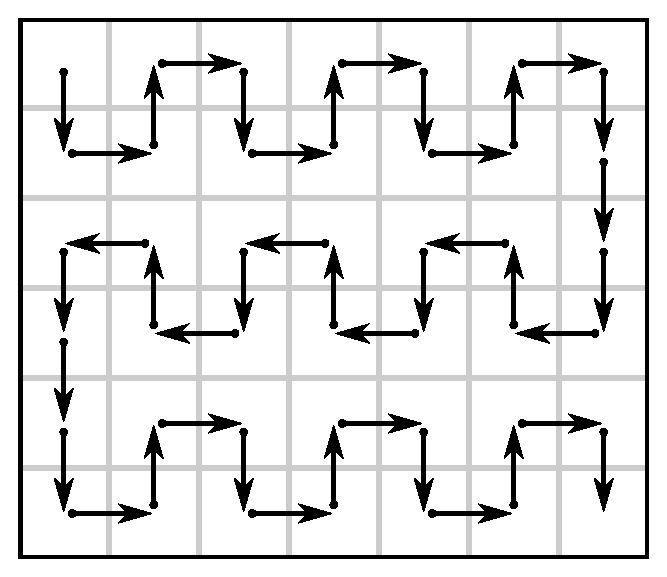
\includegraphics[width=0.3\textwidth]{figures/1threading}}}
\put(220,15){\makebox(110,85){\includegraphics[width=0.3\textwidth]{figures/2threading}}}
\end{picture}
\caption{\label{fig:threading}%
  Different ways of \emph{threading} probes on a chip. a) Standard
  row-by-row (0-threading); b) 1-threading; c) 2-threading.}%
\end{figure}

\citet{Feldman1994} were the first to formally address the unintended
illumination problem. They showed how an optimal placement can be constructed
based on a two-dimensional Gray code.  Their work, however, is restricted to
\emph{uniform arrays} (arrays containing all $4^\ell$ probes of a given length
$\ell$) and synchronous embeddings, being thus of limited practical importance
for current microarrays.

The border length problem on arrays of arbitrary probes was first
discussed by \citet{Hannenhalli2002}. The article reports that the
first Affymetrix chips were designed using a heuristic for the
traveling salesman problem (TSP). The idea is to build a weighted
graph with nodes representing probes, and edges containing the Hamming
distances between their embeddings, that is, the number of times their
embeddings differ at a particular synthesis step. A TSP tour on this
graph is heuristically constructed, resulting in consecutive probes in
the tour being likely similar. The TSP tour is then \emph{threaded} on
the array in a row-by-row fashion (Fig.~\ref{fig:threading}a).

Hannenhalli and co-workers studied several threading alternatives,
which they collectively called \emph{$k$-threading}
(Fig.~\ref{fig:threading}b,c). A $k$-threading is a variation of the
standard row-by-row threading, in which the right-to-left and
left-to-right paths are interspaced with alternating upward and
downward movements over $k$ sites. (The row-by-row threading can be
seen as a $k$-threading with $k=0$.) Hannenhalli and co-workers
experimentally observed that 1-threading may reduce border length in up to
20\% for large chips when compared to row-by-row threading.

A different strategy, called Epitaxial placement, was proposed by
\citet{Kahng2002}. It was originally designed for chips with synchronous
embeddings, but it can be trivially implemented for asynchronous embeddings as
well. The algorithm starts by placing a random probe in the center of the array
and continues to insert probes in spots adjacent to already-filled spots.
Priority is given to spots whose all four neighbors are full, in which case a
probe with the minimum number of border conflicts with the neighbors is placed.
Otherwise, all spots~$s$ with $i \geq 1$ filled neighbors are examined. For each
spot, the algorithm finds a non-assigned probe~$p$ whose number of conflicts
with the filled neighbors, $c(s,p)$, is minimal, and assigns a cost
$C(s,p) = k_i \cdot c(s,p) / i$ for this assignment, where $0 < k_i \leq 1$ are
scaling coefficients (the authors propose $k_1 = 1$, $k_2 = 0.8$, and
$k_3 = 0.6$). The assignment with minimum $C(s,p)$ is made and the procedure is
repeated until all probes have been placed. With this algorithm, Kahng and
co-workers claim a further 10\% reduction in border conflicts over
TSP\,+\,1-threading.

Both the Epitaxial algorithm and the TSP approach have at least quadratic time
complexity and hence do not scale well to large chips. This observation
motivated the design of two new placement algorithms: Sliding-Window Matching
(SWM) and Row-Epitaxial \citep{Kahng2003}.



\subsection{Sliding-Window Matching}

\begin{figure}[t!]
\centerline{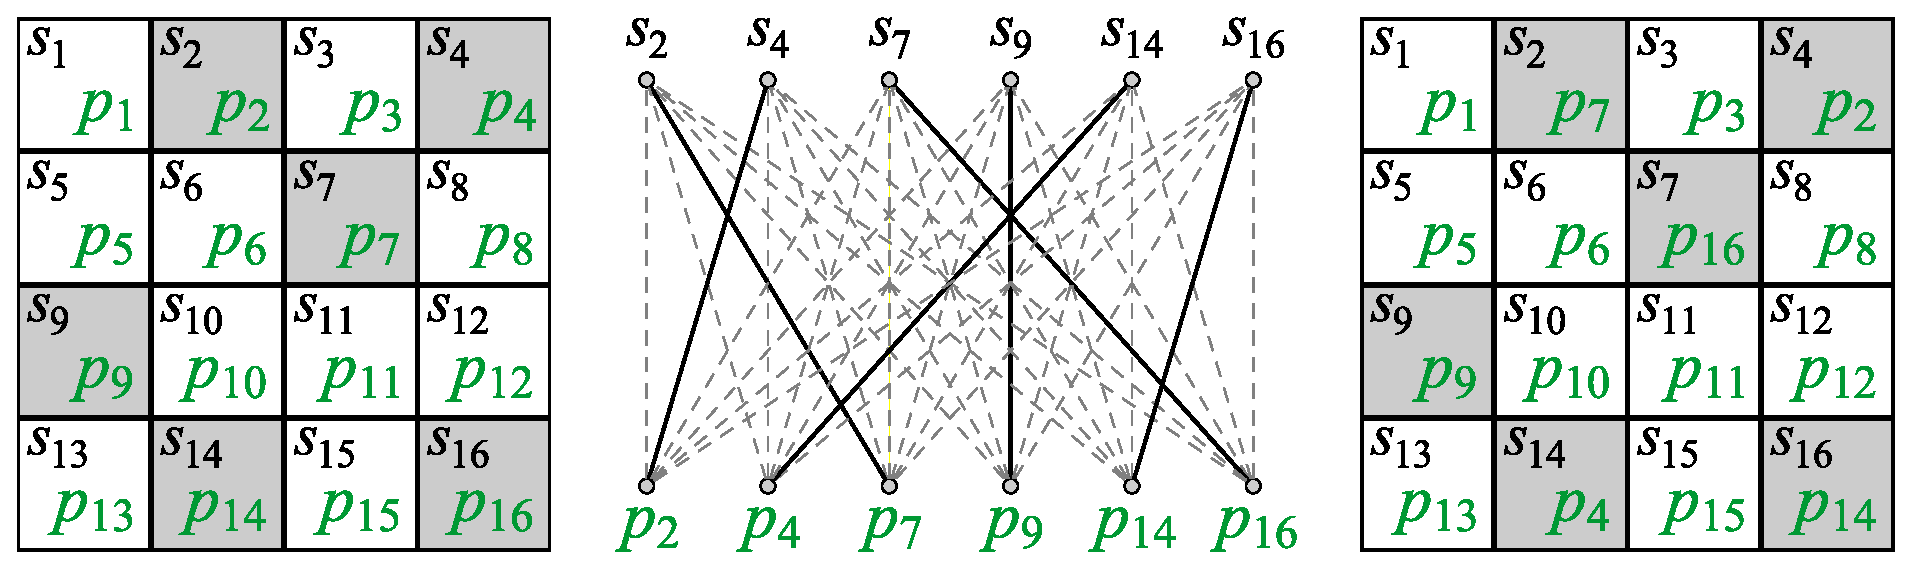
\includegraphics[width=\textwidth]{figures/swm.eps}}
\begin{picture}(340,15)
\put(0,0){\makebox(95,15){a)}}
\put(95,0){\makebox(145,15){b)}}
\put(240,0){\makebox(95,15){c)}}
\end{picture}
\caption{\label{fig:swm}%
  Sliding-Window Matching algorithm. a) Initial arrangement of probes
  $p_1 \dots p_{16}$ inside a $4 \times 4$ window and the selected independent
  set of spots (shaded). b) Bipartite graph and a minimum weight perfect
  matching (dark edges). c) New arrangement inside the window.}%
\end{figure}

The SWM is not exactly a placement algorithm as it iteratively improves an
existing placement that can be constructed, for instance, by
TSP\,+\,1-threading, or much simpler, by lexicographically sorting the binary
embedding vectors with a linear-time radix sort. The sorting is several times
faster but it is also likely to produce a worse initial placement than the
TSP, with consecutive embeddings being similar only in their first synthesis
steps. This, however, should be of little importance given that this placement
is only used as a starting point for the SWM algorithm.

The SWM works inside a window that starts at the top left of the chip
and slides from left to right, top to bottom, while maintaining a
certain amount of overlap between each iteration. When the window
reaches the right-end of the chip, it is re-started at the left-end of
the next set of rows, also retaining an overlap with the preceding
rows.

At each iteration, the algorithm attempts to reduce the total border
length inside the window by relocating some probes
(Fig.~\ref{fig:swm}a).  First, a random maximal independent set
of spots is selected, and the probes assigned to these spots are
removed. The term independent refers to the fact that selected spots
can be re-assigned to probes without affecting the border length of
other selected spots. The algorithm creates a bipartite graph with
nodes representing the removed probes and the now vacant spots
(Fig.~\ref{fig:swm}b). The edges of this graph are weighted
with the number of border conflicts that are generated by the
corresponding assignment.  Finally, a minimum weight perfect matching
on this graph is computed, and the indicated assignments are made
(Fig.~\ref{fig:swm}c).

Selecting an independent set of spots ensures that the cost of each
new assignment can be computed independently of the other assignments.
The SWM was designed for border length minimization and it takes
advantage of the fact that, in this model, an independent set of spots
can be constructed by selecting sites that are not immediate
neighbors (spots that do not share a common border).
SWM can be adapted for conflict index minimization (to our knowledge,
this has not been implemented) by using larger windows containing
relatively sparse independent sets. Therefore several random
independent sets should be constructed before moving the window.


\subsection{Row-Epitaxial}

The Row-Epitaxial algorithm is a variant of the Epitaxial algorithm
with two main differences introduced to improve scalability: i) spots
are filled in a pre-defined order, namely, from top to bottom, left to
right, and ii) only a limited number $Q$ of probes are considered
for filling each spot.

Like SWM, Row-Epitaxial improves an initial placement that is
constructed by TSP\,+\,1-threading or Radix-sort\,+\,1-threading. For
each spot $s$ of the chip, it looks at the next $Q$ probes that lie in
close proximity (to the right or below $s$), and swaps the current
probe of $s$ with the probe that generates the minimum number of
border conflicts with the top and left neighbors of $s$.
Row-Epitaxial can be adapted to conflict index minimization by
restricting the computation of the conflict index of $s$ to those
neighboring probes that are to the left or above $s$ (those which have
already found their final positions).

Fig.~\ref{fig:rowepitaxial} shows computational results for normalized border
length and average conflict index for various chip dimensions and different
values of $Q$.  The running time of Row-Epitaxial is $O(Qn)$, i.e., linear in
the chip size, where $Q$ is a user-defined constant.  In this way, solution
quality can be traded for running time: More candidates yield better layouts
but also demand more time.  For border length minimization, increasing $Q$
above 10\,000 has little positive effect.

According to experiments conducted by \citet{Kahng2003},
Row-Epitaxial is the best known large-scale placement algorithm,
achieving up to 9\% reduction in border length over the
TSP\,+\,1-threading, whereas SWM achieves slightly worse results but
requires significantly less time.


\begin{figure}
%%
\begin{picture}(334,145)\footnotesize{
  \put(0,0){\makebox(167,145){
    %GNUPLOT: LaTeX picture with Postscript
    \begin{picture}(0,0)%
    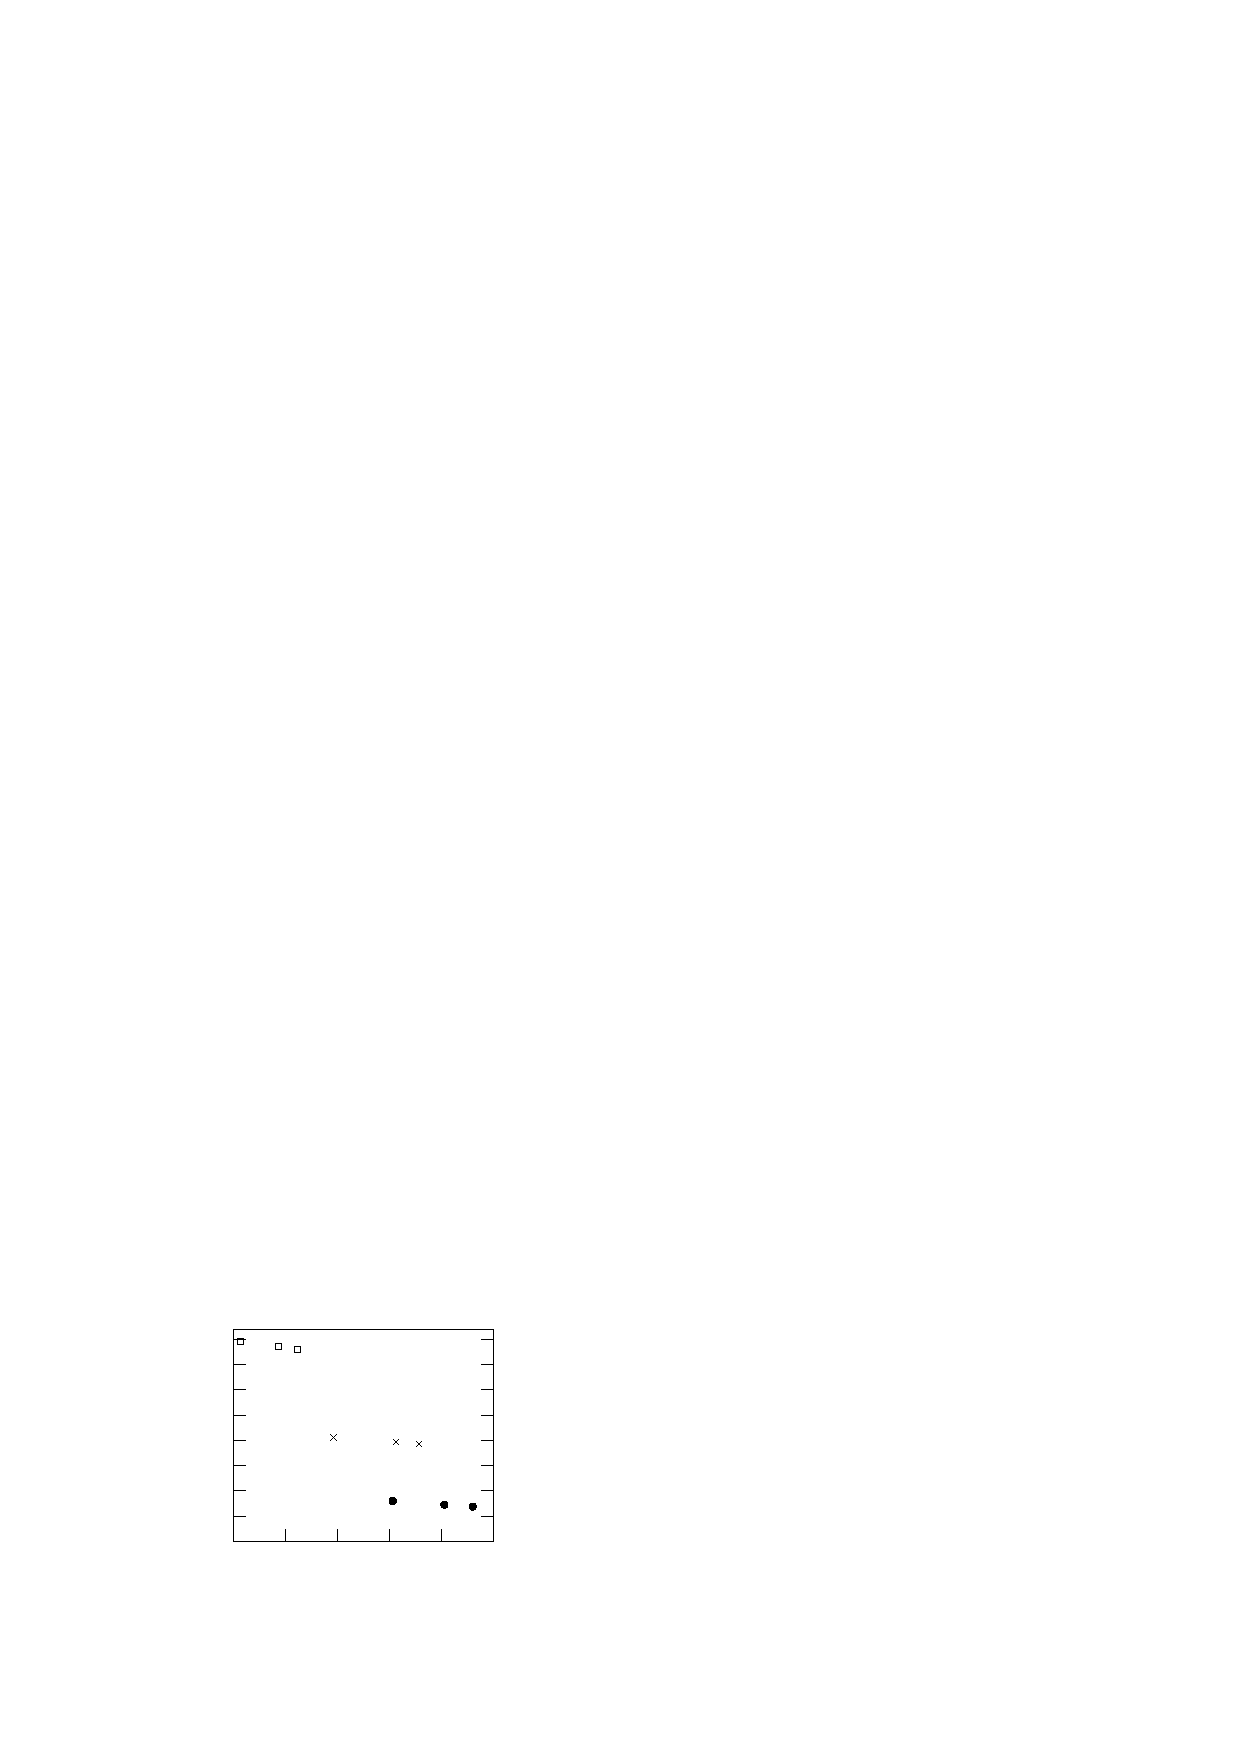
\includegraphics{figures/reptx/reptx-bl}%
    \end{picture}%
    \begingroup
    \setlength{\unitlength}{0.0200bp}%
    \begin{picture}(9000,8100)(0,0)%
    \put(1750,1500){\makebox(0,0)[r]{\strut{} 44}}%
    \put(1750,2107){\makebox(0,0)[r]{\strut{} 44.5}}%
    \put(1750,2714){\makebox(0,0)[r]{\strut{} 45}}%
    \put(1750,3321){\makebox(0,0)[r]{\strut{} 45.5}}%
    \put(1750,3929){\makebox(0,0)[r]{\strut{} 46}}%
    \put(1750,4536){\makebox(0,0)[r]{\strut{} 46.5}}%
    \put(1750,5143){\makebox(0,0)[r]{\strut{} 47}}%
    \put(1750,5750){\makebox(0,0)[r]{\strut{} 47.5}}%
    \put(1750,6357){\makebox(0,0)[r]{\strut{} 48}}%
    \put(2000,1000){\makebox(0,0){\strut{} 8}}%
    \put(3250,1000){\makebox(0,0){\strut{} 16}}%
    \put(4500,1000){\makebox(0,0){\strut{} 32}}%
    \put(5750,1000){\makebox(0,0){\strut{} 64}}%
    \put(7000,1000){\makebox(0,0){\strut{} 128}}%
    \put(8250,1000){\makebox(0,0){\strut{} 256}}%
    \put(5125,250){\makebox(0,0){\strut{}Time (min)}}%
    \put(5125,7350){\makebox(0,0){\strut{}Normalized border length}}%
    \end{picture}%
    \endgroup
  }}
  \put(167,0){\makebox(167,145){
    %GNUPLOT: LaTeX picture with Postscript
    \begin{picture}(0,0)%
    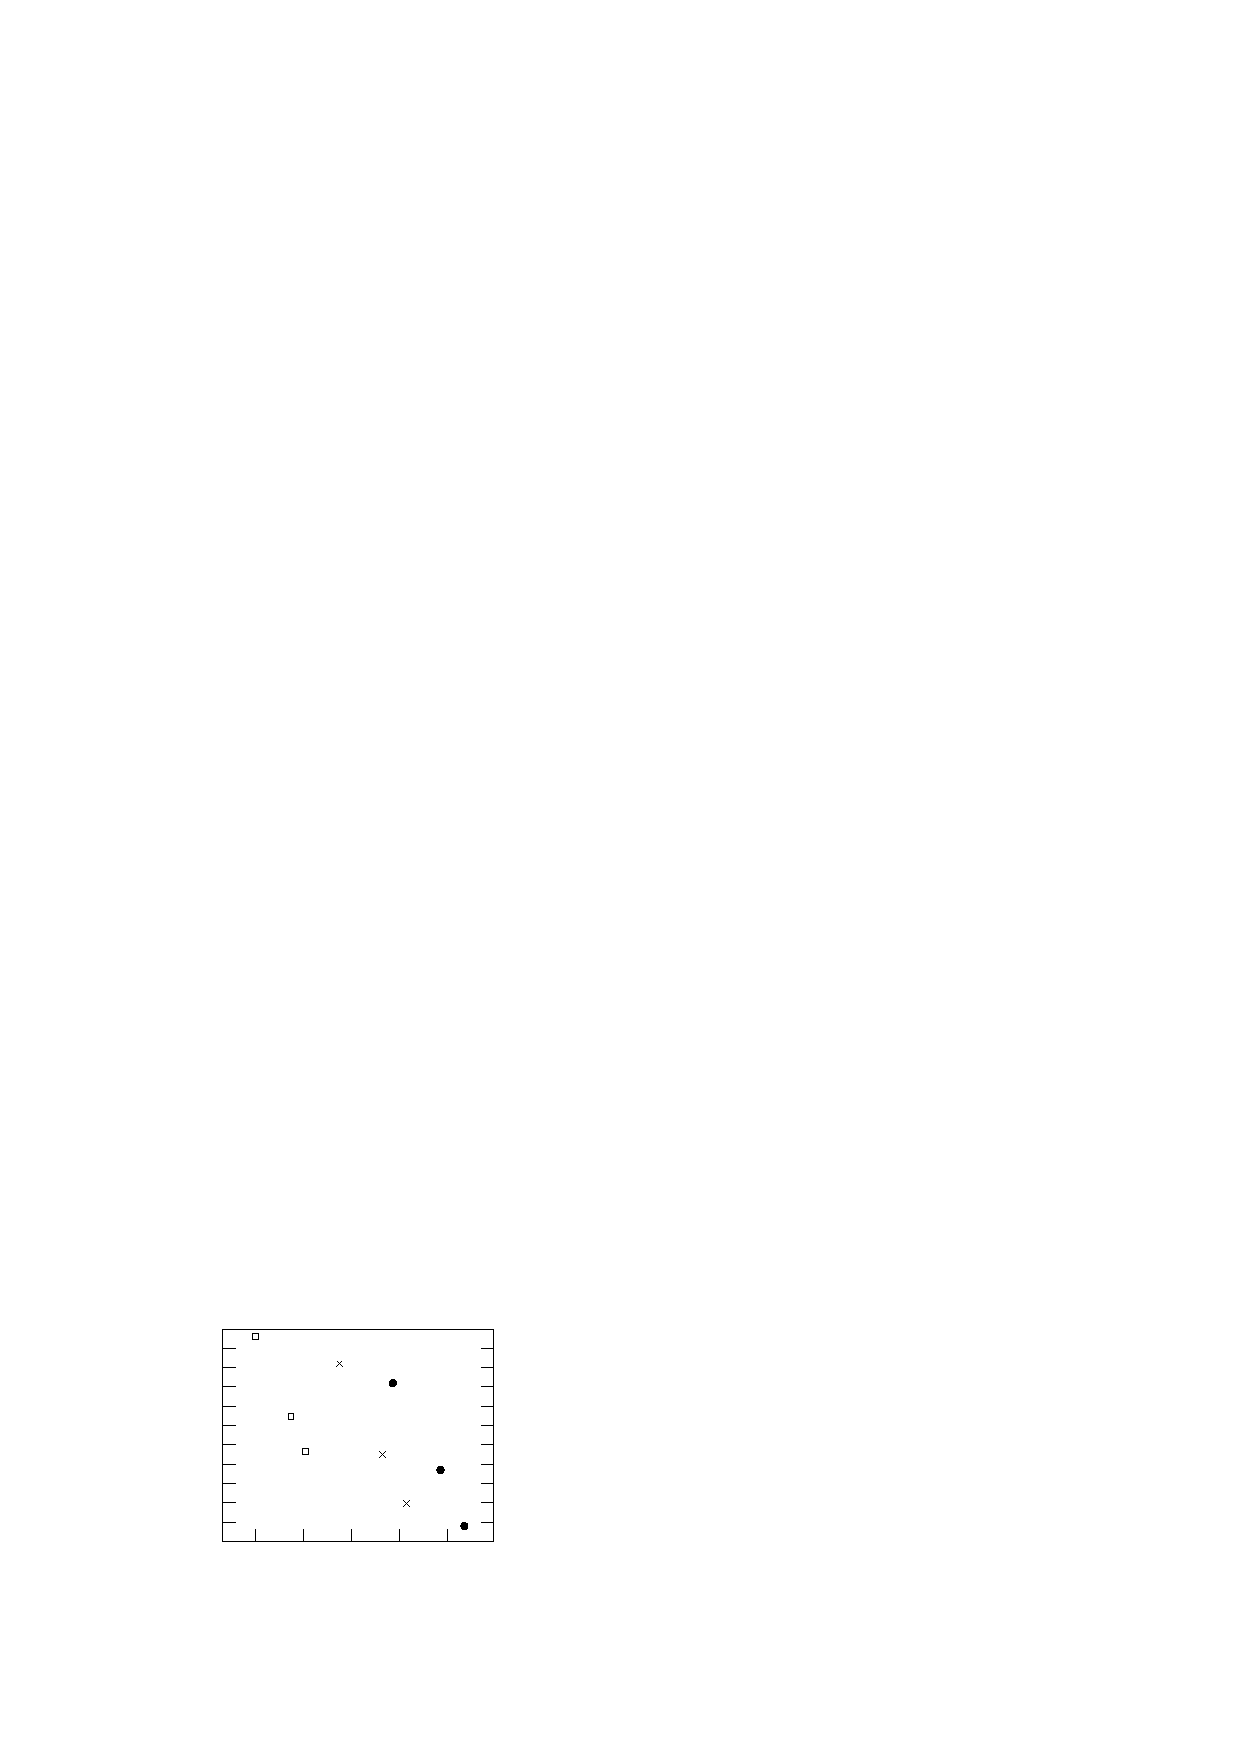
\includegraphics{figures/reptx/reptx-ci}%
    \end{picture}%
    \begingroup
    \setlength{\unitlength}{0.0200bp}%
    \begin{picture}(9000,8100)(0,0)%
    \put(1500,1500){\makebox(0,0)[r]{\strut{} 535}}%
    \put(1500,1964){\makebox(0,0)[r]{\strut{} 540}}%
    \put(1500,2427){\makebox(0,0)[r]{\strut{} 545}}%
    \put(1500,2891){\makebox(0,0)[r]{\strut{} 550}}%
    \put(1500,3355){\makebox(0,0)[r]{\strut{} 555}}%
    \put(1500,3818){\makebox(0,0)[r]{\strut{} 560}}%
    \put(1500,4282){\makebox(0,0)[r]{\strut{} 565}}%
    \put(1500,4745){\makebox(0,0)[r]{\strut{} 570}}%
    \put(1500,5209){\makebox(0,0)[r]{\strut{} 575}}%
    \put(1500,5673){\makebox(0,0)[r]{\strut{} 580}}%
    \put(1500,6136){\makebox(0,0)[r]{\strut{} 585}}%
    \put(1500,6600){\makebox(0,0)[r]{\strut{} 590}}%
    \put(2531,1000){\makebox(0,0){\strut{} 16}}%
    \put(3683,1000){\makebox(0,0){\strut{} 32}}%
    \put(4834,1000){\makebox(0,0){\strut{} 64}}%
    \put(5986,1000){\makebox(0,0){\strut{} 128}}%
    \put(7138,1000){\makebox(0,0){\strut{} 256}}%
    \put(5000,250){\makebox(0,0){\strut{}Time (min)}}%
    \put(5000,7350){\makebox(0,0){\strut{}Average conflict index}}%
    \end{picture}%
    \endgroup
  }}
}\end{picture}
%%
\caption{\label{fig:rowepitaxial}
  Trade-off between solution quality and running time with the
  Row-Epitaxial algorithm, on random chips of dimensions $200 \times
  200$ ({\tiny $\Box$}), $300 \times 300$ ({\tiny $\times$}) and $500
  \times 500$ ({\tiny $\bullet$}).  The number $Q$ of candidates per
  spot are $10\,000$, $20\,000$, and $30\,000$ from left to right.
  Layouts are measured by normalized border length (left) and average
  conflict index (right).}
\end{figure}


%%%%%%%%%%%%%%%%%%%%%%%%%%%%%%%%%%%%%%%%%%%%%%%%%%%%%%%%%%%%%%%%%%%%%%%%%%
\section{Re-embedding}
\label{sec:reembed}

Once the probes have been placed, conflicts can be further reduced by
re-embedding the probes without changing their locations. All
re-embedding algorithms presented in this section are based on the
Optimum Single Probe Embedding (OSPE) introduced by \citet{Kahng2002}.
OSPE is a dynamic programming for computing an optimum embedding of a
single probe with respect to its neighbors, whose embeddings are
considered as fixed. The algorithm was originally developed for border
length minimization but here we present a more general form designed
for the conflict index model \citep{Carvalho2006}.

\subsection{Optimum Single Probe Embedding}

The OSPE algorithm can be seen as a special case of a global alignment
between a probe sequence $p$ of length $\ell$ and the deposition
sequence $N$ of length $T$, disallowing mismatches and gaps in $N$.
We assume that $p$ is placed at spot $s$, and that we know the
embeddings of all probes placed at spots near $s$.

The optimal embedding of $p$ into $N$ is built by determining the
minimum cost of embedding a prefix of $p$ into a prefix of $N$: We use
an $(\ell + 1) \times (T + 1)$ matrix $D$, where $D[i,t]$ is defined
as the minimum cost of an embedding of $p[1..i]$ into $N[1..t]$. The
cost is the sum of conflicts induced by the embedding of $p[1..i]$ on
its neighbors, plus the conflicts suffered by $p[1..i]$ because of the
embeddings of its neighbors.

We can compute the value for $D[i,t]$ by looking at two previous
entries in the matrix: $D[i,t-1]$ and $D[i-1,t-1]$. The reason is that
$D[i,t]$ is the minimum cost of embedding $p[1..i]$ up to the
$t$-th synthesis step, which can only be obtained from the previous
step ($t-1$) by either masking or unmasking spot~$s$ at step~$t$.

If $s$ is productive at step $t$, base $N_t$ is appended to
$p[1..i-1]$; this is only possible if $p[i]=N[t]$. In this case a cost
$U_t$ is added for the risk of damaging probes at neighboring spots
$s'$. We know that $p[1..i-1]$ can be embedded in $N[1..t-1]$ with
optimal cost $D[i-1,t-1]$.  Hence, the minimum cost at step $t$, if
$s$ is productive, is $D[i-1,t-1] + U_t$.  According to the conflict
index model,
\[
U_t := \sum_{\substack{s'\text{: neighbor}\\\text{of } s}}
  \Ind{\eps_{k(s'),t}=0}
  \cdot \omega(\eps_{k(s')},t)
  \cdot \gamma(s',s).
\]


If $s$ is masked at step $t$, no base is appended to $p[1..i]$, but a
cost $M_{i,t}$ must be added for the risk of damaging $p$ (by light
directed at neighboring spots $s'$). Since $D[i,t-1]$ is the minimum
cost of embedding $p[1..i]$ in $N[1..t-1]$, the minimum cost up to step
$t$, if $s$ is unmasked, is $D[i,t-1] + M_{i,t}$.

Note that $M_{i,t}$ depends on the number of bases $p$ already
contains (that is, on $i$): Each unmasked neighboring spot $s'$
generates a conflict on $p$ with cost $\gamma(s,s') \cdot c \cdot
\exp[\theta\cdot (1+\min\{i,\ell-i\})]$, in accordance with
(\ref{eq:pos_mult})--(\ref{eq:b_ell}). Thus
\[
M_{i,t} := c \cdot \exp[\theta\cdot (1+\min\{i,\ell-i\})] \cdot
\sum_{\substack{s'\text{: neighbor}\\\text{of } s}}
\Ind{\eps_{k(s'),t}=1}  \cdot \gamma(s,s').
\]

Finally, $D[i,t]$ is computed as the minimum cost of the possible
actions,
%%
\[
D[i,t] := \begin{cases}
  \min \{\, D[i,t-1] + M_{i,t},\;  D[i-1,t-1] + U_t \,\}
  & \text{ if $p[i]=N[t]$,}\\
  D[i,t-1] + M_{i,t}
  & \text{ if $p[i]\neq N[t]$.}
  \end{cases}
\]

The first column of $D$ is initialized as follows: $D[0,0] = 0$ and
$D[i,0] = \infty$ for $0 < i \leq \ell$, since no probe of length
$\ell > 0$ can be embedded into an empty deposition sequence. The
first row is initialized by setting $D[0,t] = D[0,t-1]+M_{0,t}$ for
$0<t\leq T$.

If we assume that costs $U_t$ and $M_{i,t}$ can be computed in
constant time, the time complexity of the OSPE algorithm is $O(\ell
T)$ since there are $O(\ell T)$ entries in $D$ to compute. The algorithm can
be rather time-consuming in the general form presented here, since we
have to look at the embeddings of up to 48 neighbors around~$s$.
Naturally, it runs much faster for border length minimization, since
there are only four neighbors, and there are neither
position-dependent ($\omega$) nor distance-dependent ($\gamma$)
weights to compute. In any case, a few optimizations significantly
reduce the running time.  For instance, in each row, only the columns
between the left-most and the right-most embedding of $p$ in $N$ need
to be computed.

Once $D$ is computed, the minimum cost is $D[\ell,T]$, and an
optimal embedding of $p$ into $N$ can be constructed by tracing a path from
$D[\ell,T]$ back to $D[0,0]$, similarly to the procedure used to build an
optimal global alignment.  This takes $O(T)$ time.



\subsection{Re-embedding algorithms}

The OSPE algorithm is the basic operation of several post-placement
optimization algorithms: Greedy, Batched Greedy and Chessboard
\citep{Kahng2002}, and Sequential~\citep{Kahng2003a}. Their main difference
lies in the order in which the probes are re-embedded.

Since OSPE never increases the amount of conflicts in the region
around the re-embedded probe, optimization algorithms can execute
several re-embedding operations without risk of worsening the current
solution. Moreover, probes can be re-embedded several times since new
improvements may be possible once neighbors are changed.
In fact, the following
algorithms work in repeating cycles of optimization until no more
improvements are possible (when a local optimal solution is found), or
until improvements drop below a given threshold.
  
The Greedy algorithm uses OSPE to compute, for each spot of the chip,
the maximum reduction of border conflicts achievable by optimally
re-embedding its probe. It then selects a spot $s$ with the highest
gain (reduction of conflicts) and re-embeds its probe optimally,
updating the gains of affected neighboring spots.

A faster version of this algorithm, called Batched Greedy, pre-selects
several spots for re-embedding and thus sacrifices its greedy nature
by postponing the update of gains.

The Chessboard optimization is based on the fact that a chip can be bi-colored
like a chessboard, in such a way that the embeddings of probes located on
white spots are independent of those placed on black spots (with respect to
border length), and vice-versa. The Chessboard uses this coloring to alternate
the optimal re-embedding of probes located on black and white spots.

The Sequential optimization is the simplest algorithm among the four.
It proceeds spot by spot, from top to bottom, from left to right,
re-embedding each probe optimally. Once the end of the array is
reached, it restarts at the top left for the next iteration.

Surprisingly, the Sequential algorithm achieves the greatest reduction
of border conflicts with a running time comparable to Batched Greedy,
the fastest among the four.  All re-embedding algorithms mentioned
here were initially developed for border length minimization, but they
can all be applied to the conflict index model as well. For the
Chessboard optimization, $4\times 4=16$ colors must be used
instead of~$2$.


%%%%%%%%%%%%%%%%%%%%%%%%%%%%%%%%%%%%%%%%%%%%%%%%%%%%%%%%%%%%%%%%%%%%%%%%%%%%%%%%

\section{Partitioning}
\label{sec:partition}

We mentioned earlier that the MLP is usually approached in two phases:
placement and re-embedding. The placement, however, is sometimes
preceded by a \emph{partitioning} phase, which breaks the problem into
smaller sub-problems that are easier to manage. This is especially
helpful for placement algorithms with non-linear time or space
complexities that are otherwise unable to handle very large chips.

A partitioning algorithm divides the set of probes $\mathcal{P}$ into smaller
subsets, and assigns them to defined regions of the chip. Each region can then
be treated as an independent chip (and processed by a placement algorithm) or
recursively partitioned. Linear-time placement algorithms may also benefit from
a partitioning since probes with similar embeddings are typically assigned to
the same region (Row-Epitaxial, for instance, is more likely to find good
candidates for filling a spot).

We describe four partitioning algorithms: 1-Dimensional Partitioning,
2-Dimen\-sional Partitioning, Centroid-based Quadrisection (CQ), and
Pivot Partitioning (PP). Like placement algorithms, they assume that
an initial (left-most, right-most, synchronous or otherwise
pre-computed) embedding of the probes is given. Pivot Partitioning is
the only algorithm that modifies these embeddings.  As we shall see,
1-D and 2-D Partitioning generate a few masks with extremely few
conflicts, leaving the remaining masks with high levels of conflicts
that are difficult to handle. CQ and PP offer a more uniform
optimization over all masks. Results of \citet{Carvalho2006} indicate
that PP produces better layouts than CQ on large chips.

Partitioning is a compromise in solution quality since it restricts
the space of solutions and may lead to conflicts at partition borders.
However, it can improve solution quality in practice when the
placement algorithm cannot handle large regions well. It is not
advisable to perform too many levels of partitionings because smaller
sub-regions mean less freedom for optimization during placement. The
right balance depends on both the placement algorithm and the
partitioning algorithm.


\subsection{1-Dimensional Partitioning}

1-Dimensional Partitioning divides the set of probes based on the state of
their embeddings at a particular synthesis step. It starts by creating two
subsets of $\mathcal{P}$:
%%
\[
\mathcal{P}_0 = \{ p_k \in \mathcal{P} | \eps_{k,1} = 0 \},
\qquad
\mathcal{P}_1 = \{ p_k \in \mathcal{P} | \eps_{k,1} = 1 \}.
\]

In other words, $\mathcal{P}_0$ contains all probes whose embeddings are
unproductive during the first synthesis step, whereas $\mathcal{P}_1$
contains the probes with productive embeddings. The chip is then
divided into two horizontal bands, proportionally to the number of probes in
$\mathcal{P}_0$ and $\mathcal{P}_1$, so each band accommodates one subset
of $\mathcal{P}$.

This procedure is recursively applied to each band, using the the next
synthesis steps to further divide each subset of probes. For
instance, the following subsets of $\mathcal{P}_0$ and
$\mathcal{P}_1$ are created during step $t=2$:
%%
\[
\mathcal{P}_{00} = \{ p_k \in \mathcal{P}_0 | \eps_{k,2} = 0 \},
\qquad
\mathcal{P}_{01} = \{ p_k \in \mathcal{P}_0 | \eps_{k,2} = 1 \},
\]
\[
\mathcal{P}_{10} = \{ p_k \in \mathcal{P}_1 | \eps_{k,2} = 0 \},
\qquad
\mathcal{P}_{11} = \{ p_k \in \mathcal{P}_1 | \eps_{k,2} = 1 \}.
\]

%%%%%%%%%%%%%%%%%%%%%%
\begin{figure}\centering
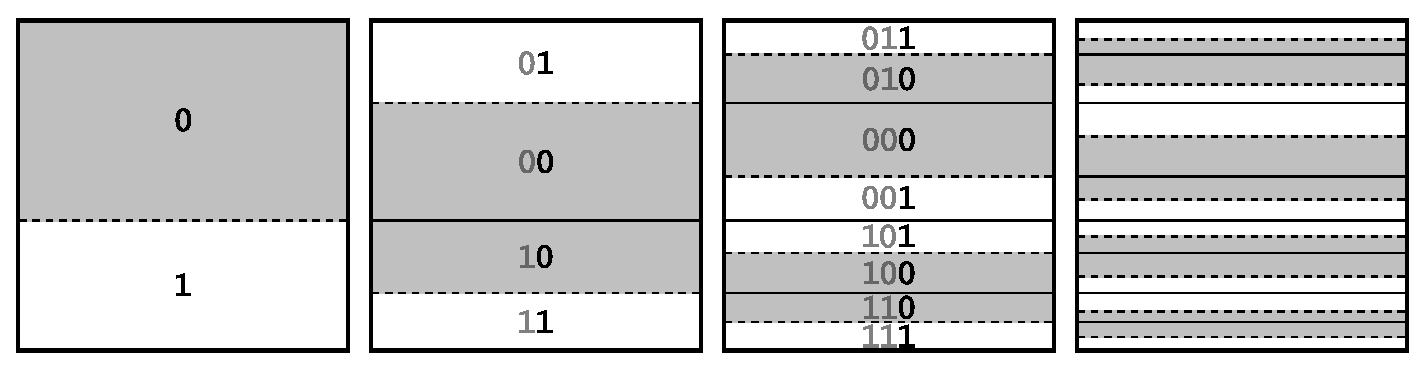
\includegraphics[width=\textwidth]{figures/1dpart.eps}
\caption{\label{fig:1dpart}%
  First four levels of 1-Dimensional Partitioning. Dashed lines show the
  divisions performed in each step; solid lines indicate regions delimited in
  previous steps (there are no border conflicts between spots separated by
  solid lines). Masked (shaded) regions are labeled ``0'',
  unmasked (white) regions are labeled ``1''. This labeling forms
  a Gray code (shown in the first three steps only).}
\end{figure}
%%%%%%%%%%%%%%%%%%%%%%%%

The next assignments of subsets to the upper or lower band of their regions
are made in such a way that regions with the same ``state'' --- productive
(unmasked) or unproductive (masked) --- are joined as far as
possible, resulting in masks that consist of alternating layers of masked and
unmasked spots. This process is illustrated in Fig.~\ref{fig:1dpart}, where at
each step~$t$, a band is labeled ``0'' when its embeddings are unproductive,
and ``1'' when its embeddings are productive. The resulting binary numbers
from top to bottom form a Gray code, i.e., two successive numbers differ in
only one bit.

The Gray code highlights an interesting property of 1-D Partitioning.
After $d$~levels of partitionings (based on steps $1$ to $d$), the
embeddings of any two immediate neighbors differ among the first
$d$~steps in at most one step.  As a result, masks $M_1 \dots M_d$
exhibit a layered structure that effectively reduces border conflicts.

Unfortunately, the Gray code is disrupted as soon as a region cannot be divided
(because all probes of that region are, for instance, masked at a particular
step). This will certainly happen as several binary numbers are unlikely to be
substrings of embeddings (think of, for example, a long run of zeros).

Moreover, 1-D Partitioning can optimize only a limited number of masks
because the sub-regions soon become too narrow to be further divided. The
maximum \emph{partitioning depth} $d_{max}$ is primarily limited by the number
of rows in the chip. In practice, since regions are likely to be unevenly
divided, $d_{max}$ varies between regions. The algorithm can also be configured
to stop partitioning a region once its dimensions drop below a given threshold.

1-D Partitioning is easier to implement if the partitionings always produce
rectangular regions (i.e., splitting a row between two regions is not allowed).
In order to force an exact division of a region, however, it might be necessary
to move a few probes from one subset of probes to the other one.

%%
%% OPTIONAL: could be removed to save space
%%
\optional{%
For example, imagine that a chip with $|\mathcal{P}| = 900$ probes, $n_r = 30$
rows and $n_c = 30$ columns is to be partitioned based on the state of the
embeddings at the first synthesis step, resulting in sub-sets $\mathcal{P}_0$
and $\mathcal{P}_1$ with, say, 638 and 262 probes, respectively. The chip must
thus be divided into two sub-regions, the upper one containing $[30 \cdot
638/900]=21$ rows and the lower one with $[30 \cdot 262/900]=9$ rows ($[x]$ is
$x$ rounded to the nearest integer). The problem is that the upper region then
contains $21 \cdot 30 = 630$ spots but it has to accommodate 638 probes,
whereas the lower region contains $9 \cdot 30 = 270$ spots but only 262
probes. The solution is to (arbitrarily) move 8 probes from $\mathcal{P}_0$ to
$\mathcal{P}_1$, which, results in some imperfections in the layers
of the corresponding mask (a few masked spots in a region of unmasked spots,
for instance).
}


\subsection{2-Dimensional Partitioning}

%%%
\begin{figure}\centering
\includegraphics[width=\textwidth]{figures/2dpart.eps}
\caption{\label{fig:2dpart}%
  First four levels of 2-Dimensional Partitioning. Dashed lines show
  the divisions performed in each step; solid lines indicate regions
  delimited in previous steps. Masked regions are labeled with ``0'',
  unmasked regions with ``1''; this labeling forms an approximation to
  a two-dimensional Gray code.}%
\end{figure}
%%%

The 2-Dimensional Partitioning algorithm extends the idea of 1-D
Partitioning to two dimensions, with the potential of optimizing twice
as many masks. The algorithm is similar: $\mathcal{P}$ is divided into
subsets based on the state of the embeddings at a particular
synthesis step. The difference is that 2-D Partitioning alternates
horizontal and vertical divisions of regions, and that the assignments
of probes to regions obey a two-dimensional Gray code
(Fig.~\ref{fig:2dpart}).

In a 2-D Gray code, two neighboring numbers differ in at most one
bit.  Thus, regions whose embeddings are at the same state (productive or
unproductive) are joined as far as possible.

If regions were always equally divided, 2-D Partitioning would have
the same property as 1-D Partitioning: After $d$~levels of
partitionings (based on steps $1$ to $d$), the embeddings of any two
immediate neighbors would differ among the first $d$ steps in at most
one step. However, this is not always the case since 2-D Partitioning
is likely to create regions with different dimensions, forcing some
regions to share a border with more than its four natural neighbors
(for example, region ``1100'' in Fig.~\ref{fig:2dpart} borders with
``0101'' and ``1111'').

So far we have described both 1-D and 2-D Partitionings using the
state of the first $d$ synthesis steps to divide the set of probes.
The result of this approach is that, while the first masks are
optimized, the remaining masks are left with high levels of border
conflicts; we call this a \emph{left-most mask optimization}.

However, a defect in the middle of the probe is more harmful than in
its extremities, so it is more important to optimize the central masks,
which synthesize the middle bases. Thus we
partition the chip based on the following sequence
of synthesis steps, assuming that $T$ is even and $d$ is odd: $T/2,
(T/2)\pm 1, (T/2)\pm 2, \dots, (T/2)\pm\lfloor d/2\rfloor$; we call
this a \emph{centered mask optimization}.

For left-most optimization, it makes sense to embed the probes in a
left-most fashion in order to reduce conflicts in the last masks
(which are not optimized by the partitioning); the left-most
embeddings reduce the number of unmasked spots in the last steps,
resulting in masks that largely consist of masked spots. Similarly,
centered mask optimization produces better results with \emph{centered
  embeddings}. A centered embedding is constructed by shifting a
left-most embedding to the right so that the number of masked steps to
the left of the first productive step approximately equals the number
of masked steps to the right of the last productive step.

%%%
\begin{figure}\centering
%%
\begin{picture}(335,150)\footnotesize{
  \put(0,0){\makebox(335,150){
    %GNUPLOT: LaTeX picture with Postscript
    \begin{picture}(0,0)%
    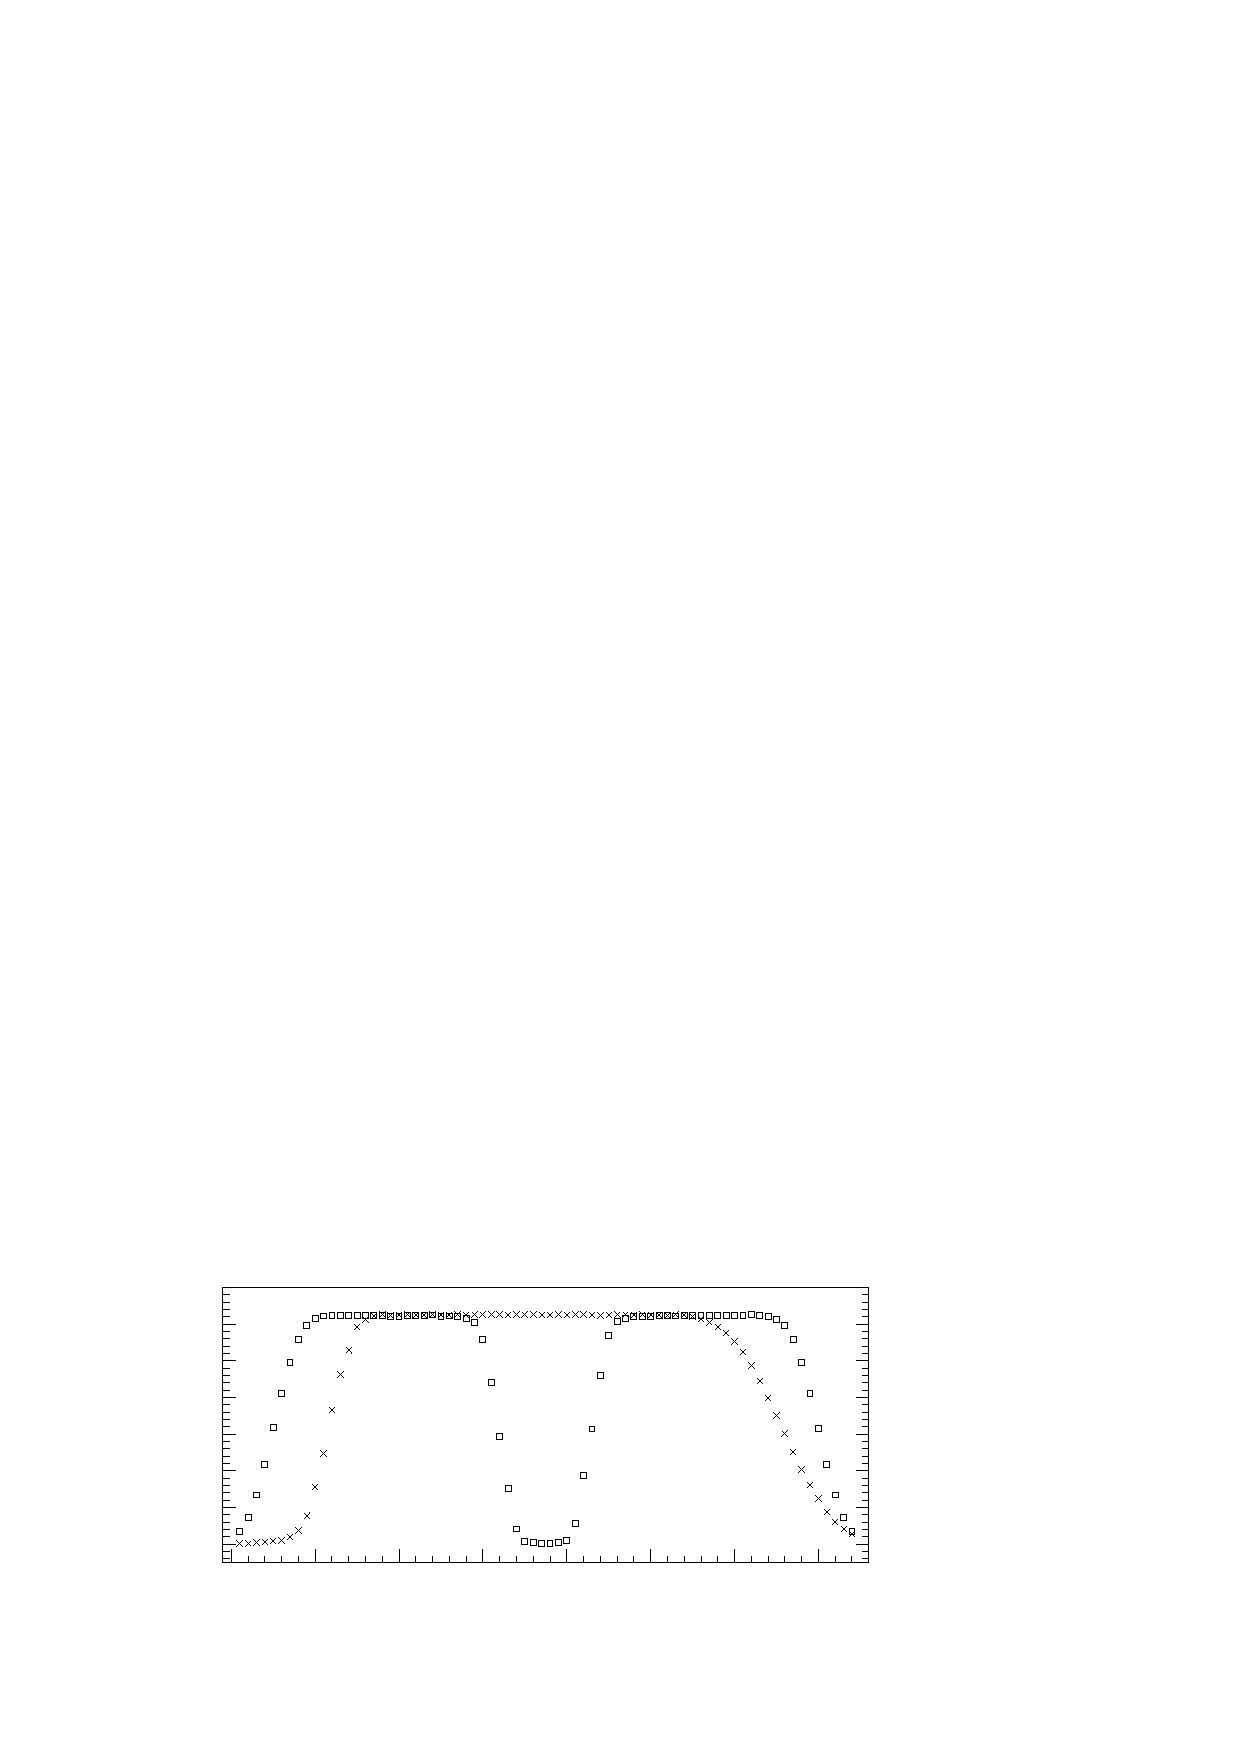
\includegraphics{figures/2dpart_bl/2dpart_bl}%
    \end{picture}%
    \begingroup
    \setlength{\unitlength}{0.0200bp}%
    \begin{picture}(18000,8100)(0,0)%
    \put(1500,1440){\makebox(0,0)[r]{\strut{} 0}}%
    \put(1500,2320){\makebox(0,0)[r]{\strut{} 0.1}}%
    \put(1500,3200){\makebox(0,0)[r]{\strut{} 0.2}}%
    \put(1500,4080){\makebox(0,0)[r]{\strut{} 0.3}}%
    \put(1500,4960){\makebox(0,0)[r]{\strut{} 0.4}}%
    \put(1500,5840){\makebox(0,0)[r]{\strut{} 0.5}}%
    \put(1500,6720){\makebox(0,0)[r]{\strut{} 0.6}}%
    \put(1500,7600){\makebox(0,0)[r]{\strut{} 0.7}}%
    \put(1951,500){\makebox(0,0){\strut{} 0}}%
    \put(3964,500){\makebox(0,0){\strut{} 10}}%
    \put(5977,500){\makebox(0,0){\strut{} 20}}%
    \put(7990,500){\makebox(0,0){\strut{} 30}}%
    \put(10003,500){\makebox(0,0){\strut{} 40}}%
    \put(12016,500){\makebox(0,0){\strut{} 50}}%
    \put(14029,500){\makebox(0,0){\strut{} 60}}%
    \put(16042,500){\makebox(0,0){\strut{} 70}}%
    \end{picture}%
    \endgroup
  }}
}\end{picture}
%%
%\includegraphics[width=\textwidth]{2dpart.eps}
\caption{\label{fig:2dpart_bl}%
  Normalized border length (on the y-axis) per masking step (on the x-axis) of
  a layout produced by 2-Dimensional Partitioning for a $1\,000 \times 1\,000$
  chip with random probe sequences (embedded in the standard 74-step Affymetrix
  deposition sequence). Partitioning stops when a region becomes smaller than
  $64 \times 64$; Row-Epitaxial is used for the placement. ({\tiny $\times$})
  Left-most mask optimization with left-most embeddings; ({\tiny $\Box$})
  centered mask optimization with centered embeddings.}
\end{figure}
%%%

Fig.~\ref{fig:2dpart_bl} shows the results of 2-D Partitioning on a
$1\,000\times 1\,000$ chip with both optimizations. For left-most mask
optimization, we obtain a normalized border length of 33.89 (up to
approximately 0.6 per step). For centered mask optimization, the normalized
border length improves slightly to 33.59. The average conflict index (not
shown in the figure) for left-most mask optimization is 571.8; for centered
mask optimization, it improves considerably to 383.5 because of the higher
weight of the middle bases.


\subsection{Centroid-based Quadrisection}

\optional{%
\begin{figure}\centering
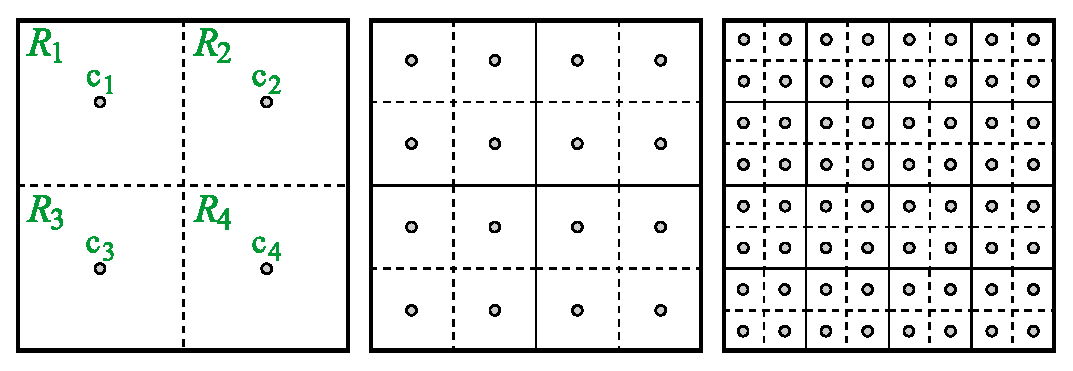
\includegraphics[width=\textwidth]{figures/quadrisect.eps}
\caption{\label{fig:quadrisect}%
  First three levels of Centroid-base Quadrisection Partitioning. Dashed lines
  show the divisions performed in each step; solid lines indicate regions
  delimited in previous steps. The centroids of each partition $R_1 \dots R_4$
  are represented by small circles (labeled with $q_1 \dots q_4$ in the first
  step).}
\end{figure}
}

Centroid-based Quadrisection or CQ \citep{Kahng2003a} employs a
different criterion for dividing the set of probes and a different
approach for partitioning. At each iteration, a region $R$ is
quadrisectioned into $R_1$, $R_2$, $R_3$, and $R_4$. Each sub-region
$R_i$ is associated with a selected probe $p_{c_i}\in \mathcal{P}$,
called \emph{centroid}, that is used to guide the assignment of the
remaining probes to the sub-regions.

A centroid is a representative of its region; it should symbolize the
``average embedding'' in that region. The remaining probes $p_k \in
\mathcal{P} \setminus \{p_{c_1},p_{c_2},p_{c_3},p_{c_4}\}$ are
compared to each centroid and assigned to the sub-region $R_i$ whose
centroid's embedding $\eps_{c_i}$ has minimum $H(k,c_i)$, where
$H(k,k')$ is the Hamming distance between the embeddings $\eps_k$ of
$p_k$ and $\eps_{k'}$ of $p_{k'}$ (i.e., the number of steps in which
$\eps_k$ and $\eps_{k'}$ differ).

In order to improve the clustering of similar probes, the four
centroids should be very different from each other. The following
heuristic is used: First, a probe index $c_1$ is randomly selected
from $\{1,\dots,|\mathcal{P}|\}$.  Then, a probe index $c_2\neq c_1$
maximizing $H(c_2,c_1)$ is selected.  Similarly, $c_3$ maximizing
$H(c_3,c_1) + H(c_3,c_2)$ and $c_4$ maximizing $H(c_4,c_1) +
H(c_4,c_2) + H(c_4,c_3)$ are selected.  The assignment of centroids to
the quadrisections of the chip is arbitrary.

In order to recover from a possibly bad choice of centroids, one can
use a ``multi-start heuristic'', running the centroid selection
procedure several times (using different ``seeds'' for $c_1$), and
keeping those that lead to the best partitioning (partitioning quality
is measured by the sum of Hamming distances of probe embeddings to
their corresponding centroid embeddings).

The partitioning continues recursively until a pre-defined depth has been
reached.

CQ was developed for border length minimization, but can be adapted
for conflict index minimization by using the \emph{conflict index
  distance} $C(k,k')$ instead of the Hamming distance $H(k,k')$
between the embeddings $\eps_k$ and $\eps_{k'}$,
%%
\begin{equation}
\label{eq:ci_dist}
C(k,k') := \sum_{t=1}^{T}
  \Bigl(
    \Ind{\eps_{k,t}=0 \text{ and } \eps_{k',t}=1}
    \cdot \omega(\eps_{k},t)
    +
    \Ind{\eps_{k',t}=0 \text{ and } \eps_{k,t}=1}
    \cdot \omega(\eps_{k'},t)
  \Bigr).
\end{equation}
%%
It can be interpreted as the sum of the conflict indices resulting
from placing probes $p_k$ and $p_{k'}$ at hypothetical neighboring
spots, ignoring the distance between these spots and the conflicts
generated by other neighbors.


\subsection{Pivot Partitioning: Merging partitioning and re-embedding}

Pivot Partitioning or PP \citep{Carvalho2006} is, to a certain extent,
similar to CQ: Sub-regions are recursively associated with special
probes $p_{c_i}$, here called \emph{pivots} instead of centroids, that
are used to guide the assignment of the other probes to the
sub-regions.  The main differences between PP and CQ are as follows.

Instead of quadrisectioning the chip, PP creates sub-regions by
alternating horizontal and vertical divisions (like 2-D Partitioning).
The advantage is that regions are divided proportionally to the size
of each subset of probes, so they are not required to have the same
size. Furthermore, for each partitioning level, only two pivots need
to be selected.

Another distinction is motivated by the fact that different probes
have different numbers of embeddings, ranging from a single one to
several millions.  Probes with more embeddings can more easily adapt
to the other probes, that is, they are more likely to have an
embedding with fewer conflicts to fill a particular spot than a probe
that has only a limited number of embeddings. For this reason, PP uses
probes with a single embedding (or few embeddings) as pivots, and
chooses the other probes' embeddings and region assignments accordingly.

Indeed, the most important feature of PP is the simultaneous embedding and
assignment of probes to sub-regions. Let $M(k,c_i)$ denote the minimum
conflict index distance $C(k,c_i)$, as defined in~(\ref{eq:ci_dist}), over all
embeddings of $p_k$; we call it the \emph{minimum conflict index distance}
between probes $p_k$ and $p_{c_i}$. It can be efficiently computed with a
variant of the OSPE algorithm that ignores the location of the probes and the
distance-dependent weights $\gamma$. Now, a non-pivot probe $p_k$ is assigned
to the region $R_i$ whose pivot $p_{c_i}$ has minimum $M(k,q_i)$ over $i=1,2$.
Pivot Partitioning continues recursively up to a pre-defined depth. Finally,
each probe is embedded to minimize conflicts with its assigned pivot.


%%%%%%%%%%%%%%%%%%%%%%%%%%%%%%%%%%%%%%%%%%%%%%%%%%%%%%%%%%%%%%%%%%%%%%%%%%%%%%%%
\section{Merging Placement and Re-embedding}
\label{sec:merging}

The problem with the traditional ``place and re-embed'' approach is that the
arrangement of probes on the chip is decided based on embeddings that are
likely to change during the re-embedding phase. Intuitively, better results
should be obtained when the placement and embedding phases are considered
simultaneously instead of separately. However, because of the generally high
number of embeddings of each single probe, it is not easy to design algorithms
that efficiently use the additional freedom and run reasonably fast in
practice.

We describe \Greedyplus, the first placement algorithm that simultaneously
places and re-embeds the probes, and compare it with Row-Epitaxial, the best
known large-scale placement algorithm.


\subsection{\Greedyplus}

The goal is to design an algorithm that is similar to Row-Epitaxial, so that we
can make a better assessment of the gains resulting from merging the placement
and re-embedding phases.

\Greedyplus\ fills the spots row-by-row, from left to right, in a
greedy fashion, similarly to Row-Epitaxial. Also, for each spot $s$,
it looks at $Q$ probe candidates and chooses the one that can be
placed at $s$ with minimum cost. The difference is that we now
consider all possible embeddings of a candidate $p$ instead of only
$p$'s initial embedding. This is done by temporarily placing $p$ at
$s$ and computing its optimal embedding with respect to the
already-filled neighbors of $s$ (using OSPE from
Sec.~\ref{sec:reembed}).

Compared to Row-Epitaxial, \Greedyplus\ spends more time evaluating each probe
candidate $p$ for a spot $s$. While Row-Epitaxial takes $O(T)$ time to compute
the conflict index or the border length resulting from placing $p$ at $s$,
\Greedyplus\ requires $O(\ell T)$ time since it uses OSPE (recall that $\ell$
is the probe length and $T$ is the length of the deposition sequence). To
achieve a running time comparable to Row-Epitaxial, we must therefore consider
lower candidate numbers $Q$.

There are a few optimizations that reduce the time spent with OSPE
computations when several probe candidates are examined in succession
for the same spot. First, we note that if two probe candidates $p$ and
$p'$ share a common prefix of length $l$, the first $l + 1$ rows of
the OSPE dynamic programming matrix $D$ will be identical. In other
words, if we have calculated the minimum cost of $p$, we can speed up
the calculation of the minimum cost of $p'$ by skipping the first $l +
1$ rows of $D$.

In order to fully exploit this fact, we examine the probes in
lexicographical order so that we maximize the length of the common
prefix between two consecutive candidates. We keep a doubly-linked
list of probes and remove a probe $p$ from the list when it is placed.
For the next spot to be filled, we look at $Q$ probes in the list
around $p$'s former position, e.g., at $Q/2$ probes to the left and to
the right of $p$.

Second, the $U_t$ costs of OSPE need to be computed only once for a given spot
$s$ since $U_t$ does not depend on the probe placed at $s$. Thus, in order to
examine another candidate, we only need to recompute the $M_{i,t}$ costs.

Finally, once we know that a probe candidate $p$ can be placed at $s$
with minimum cost $C$, we can stop the OSPE computation for another
candidate $p'$ as soon as all values in a row of $D$ are greater than
or equal to $C$.


\subsection{Results}

\begin{table}[t!]\centering
\caption{\label{tab:reptxplus}\boldmath%
  Normalized border length (NBL) and average conflict index (ACI) 
  of layouts produced by Row-Epitaxial and \Greedyplus\ placement (Pl.), 
  followed by Sequential re-embedding (Re-emb.)
  with thresholds $W = 0.1\%$ for border length minimization
  and $W = 0.5\%$ for conflict index minimization. $Q$ is the number of
  probe candidates considered for each spot during placement.
  Running times are given in seconds.}
\vspace*{1ex}
\begin{tabular*}{\hsize}{lrrrr}  % formerly {@{\extracolsep{\fill}}lrrrr}
\hline
\textbf{Border length min.} & \multicolumn{2}{c}{$335 \times 335$ (E.Coli)} & \multicolumn{2}{c}{$515 \times 515$ (Maize)} \cr
\hline
\textbf{Row-Epitaxial.}\; $Q$ &    10 K &   20 K   &  10 K     &  20 K    \cr
Time (Pl. + Re-emb.)     & 629 + 9 & 1211 + 9 & 3333 + 38 & 6806 + 38\cr
NBL (Pl.)                & 34.11   & 33.81    & 33.11     & 32.87    \cr
NBL (Pl. + Re-emb.)      & 33.93   & 33.66    & 32.95     & 32.73    \cr
\hline
\textbf{\Greedyplus.}\; $Q$            & 350     &   700    &   350     &    700   \cr
Time (Pl. + Re-emb.)     & 596 + 12& 1158 + 12& 2633 + 53 & 4974 + 53\cr
NBL (Pl.)                & 33.79   & 33.22    & 33.07     & 32.38    \cr
NBL (Pl. + Re-emb.)      & 33.53   & 32.98    & 32.82     & 32.16    \cr
\hline
\cr
\hline
\textbf{Conflict index min.} & \multicolumn{2}{c}{$335 \times 335$ (E.Coli)} & \multicolumn{2}{c}{$515 \times 515$ (Maize)} \cr
\hline
\textbf{Row-Epitaxial.}\; $Q$ & 5 K        & 10 K        & 5 K         & 10 K       \cr
Time (Pl. + Re-emb.)          & 930 + 1169 & 1732 + 1167 & 4082 + 4424 & 7856 + 4415\cr
ACI (Pl.)                     & 584.92     & 544.93      & 604.04      & 574.68     \cr
ACI (Pl. + Re-emb.)           & 544.23     & 514.10      & 554.87      & 532.74     \cr
\hline
\textbf{\Greedyplus.}\; $Q$ &    200 &     300 &    200 &    300 \cr
Time (Pl. + Re-emb.)        & 522 + 788 & 685 + 788 & 2131 + 2926 & 2757 + 2930\cr
ACI (Pl.)                   & 462.52 &  450.15 & 459.38 & 446.76 \cr
ACI (Pl. + Re-emb.)         & 458.02 &  445.98 & 454.84 & 442.55 \cr
\hline
\end{tabular*}
\end{table}

We compare the results of \Greedyplus\ with Row-Epitaxial. To be fair,
since Row-Epitaxial is a traditional placement algorithm that does not
change the embeddings, we need to compare the layouts obtained by both
algorithms after a re-embedding phase. For this task we use the
Sequential algorithm (Sec.~\ref{sec:reembed}) with
thresholds of $W=0.1\%$ for border length minimization and $W=0.5\%$
for conflict index minimization, so that the algorithm stops as soon
as the improvement in one iteration drops below $W$.

Table~\ref{tab:reptxplus} shows the total border length and the
average conflict index of layouts produced by both algorithms on two
chips with dimensions $335 \times 335$ and $515 \times 515$, filled
with probes randomly selected from existing GeneChip arrays (E.Coli
Genome 2.0 and Maize Genome, respectively). Probes are initially
left-most embedded into the standard 74-step Affymetrix deposition
sequence \{TGCA\}$^{18}$TG. The parameter $Q$ is chosen differently
for both algorithms so that the running time is approximately
comparable (e.g., for border length minimization, $Q=350$ for
\Greedyplus\ corresponds to $Q=10\,000$ for Row-Epitaxial). We make
the following observations.

First, increasing $Q$ linearly increases placement time, while only
marginally improving chip quality for border length minimization.

Second, re-embedding runs very quickly for border length minimization,
even on the larger chip. For conflict index minimization, the time for
the re-embedding phase exceeds the time for the placement phase for
both algorithms.

Finally, \Greedyplus\ always produces better layouts in the same amount of
time (or less) while looking at fewer probe candidates.  In particular, for
conflict index minimization on the $515\times 515$ chip with $Q=5\,000$ resp.\ 
$200$, \Greedyplus\;and Sequential improve the average conflict index by 18\%
(from 554.87 to 454.84) and need only 60\% of the time, compared to
Row-Epitaxial and Sequential.


%%%%%%%%%%%%%%%%%%%%%%%%%%%%%%%%%%%%%%%%%%%%%%%%%%%%%%%%%%%%%%%%%%%%%%%%%%%%%%%%
\section{Summary}
\label{sec:summary}

We have surveyed algorithms for the microarray layout problem (MLP), divided
into placement, (re-)embedding, and partitioning algorithms.  Because of the
super-exponential number of possible layouts and the relation to the quadratic
assignment problem (QAP), we cannot expect to find optimal solutions. Indeed,
the algorithms we present are heuristics with an emphasis on good scalability
and ideally a user-controllable trade-off between running time and solution
quality, albeit without any known provable guarantees.

Among the presented approaches, two recent ones (Pivot Partitioning and
\Greedyplus) indicate that the traditional ``place first and then re-embed''
approach can be improved upon by merging the partitioning/placement and
(re-)embedding phases. Ongoing work will show the full potential of such
combined approaches.


\ignore{As a suggestion for further work, we note the needed for improving
  the selection of probe candidates considered for filling each spot. For
  example, instead using a sorted list of probes, one could use a TSP tour
  like the early algorithms described in Sec.~\ref{sec:placement}. However,
  it is not clear if the more time-consuming TSP approach will pay off
  (instead, we could use this extra time to look at more candidates).
  
  An alternative that sounds interesting would be to build some kind of
  ``clustering'' of the probes, perhaps based on a graph or a tree, in such a
  way that we can find similar probes more easily and spend time on candidates
  that are more likely to produce less conflicts.%
}


%%%%%%%%%%%%%%%%%%%%%%%%%%%%%%%%%%%%%%%%%%%%%%%%%%%%%%%%%%%%%%%%%%%%%%%%%%%%%%%%

%% optional
%\begin{acknowledgments}
%...
%\end{acknowledgments}

%%% References should come before appendices unless there is
% a reference cite in the appendix, in which case references
% should come after the appendices.

%% Necessary! Either
%\begin{references}
%\bibitem{label}text...
%\end{references}

% or if you are using BibTeX:
\bibliographystyle{apalike}
\chapbblname{chiplayout}
\chapbibliography{chiplayout}

%% appendix optional
%\appendix{This is the Appendix Title}
%This is an appendix with a title.

%\appendix{}
%This is an appendix without a title.


\end{document}

